\begin{savequote}[8cm]
\textlatin{Neque porro quisquam est qui dolorem ipsum quia dolor sit amet, consectetur, adipisci velit...}

There is no one who loves pain itself, who seeks after it and wants to have it, simply because it is pain...
  \qauthor{--- Cicero's \textit{de Finibus Bonorum et Malorum}}
\end{savequote}

\chapter{\label{ch:5-tki}TKI} 

\minitoc

\section{in ND up}


       Neutrino-nucleus interaction is an overarching term including complicated effects besides the most fundamental neutrino-nucleon interaction. 
       First of all, the nucleons in the nucleus have different initial nuclear states (IS). 
       There is no way to determine their kinematics before its interaction with the neutrino. 
       They can only be estimated from nuclear models, which have no definitive answers and are still hot topics of current research. 
       Moreover, there could be correlation between a pair of nucleons such that the interaction between a neutrino and one nucleon can affect another nucleon significantly as well. Last but not least, after the neutrino-nucleon interaction, the final products are still inside the nucleus. 
       On their way out, it is not uncommon that they interact with the nuclear medium on their way out of the nuclei so that their kinematics are drastically altered. 
       These are the so-called Final State Interactions (FSI). 
       After they leave the nucleus, they can then be detected by our detectors if they possess energy above the detection threshold. 
       Hence, measurements of particle kinematics from the neutrino-nucleus interaction are unavoidably a convolution of all these effects, each approximated by a model. 
    
        \begin{figure}[!htb] 	
            \centering 		
            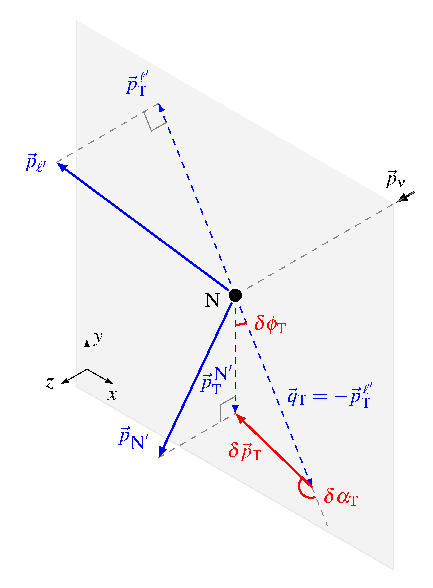
\includegraphics[width=0.35\textwidth]{fig/stki.eps}
            \caption{\label{fig:stki} Schematic illustration of the TKI variables. Diagram taken from Ref.~\cite{Lu:2015tcr}.} 
        \end{figure}
    
       The TKI variables are shown in Fig.~\ref{fig:stki}. They are cleverly constructed such that they are most sensitive to IS and FSI. 
       In the simplest case, there are only two final particles after the neutrino-nucleon interaction, a muon and a proton. 
       If the initial momentum of the struck nucleon has no component transverse to the neutrino's incoming direction, the products, i.e. the muon and the proton, should not have a net transverse component either, unless the struck nucleon has a non-zero initial transverse component or the final particles have undergone FSI.
       Suppose there is no FSI, the net transverse component, $\dpt$, corresponds exactly to the magnitude of the transverse component of the struck nucleon, and the angle, $\dat$, represents the direction of the initial nucleon motion projected on the transverse plane. 
       Assuming the nucleons are moving isotropically, the $\dat$ distribution should be flat. 
       All current nuclear models do not have a preferential direction for initial nuclear motion, so it is only natural to assume the nucleons move in random directions. 
       Thus, the deviation from flatness for $\dat$ can only be due to FSI, thereby making it an excellent probe for FSI. 
       As for $\dpt$, it reflects the magnitude of the initial nucleon momentum transverse to the neutrino direction compounded by FSI. 
       Furthermore, if the nucleus is assumed to be at rest and no other particles are knocked out other than the muon and the proton, the initial nucleon momentum, $\pn$, can also be derived following the steps outlined in \cite{pnpaper}. 
    

    \subsection{TKI in $\numucczpiop$ selection}
    
        To make a measurement of the TKI variable, an event selection needs to be made.
        At ND280, the protons from the primary neutrino interaction do not travel far and are usually contained in SFGD. 
        Hence, the $\numucczpiop$ presented in this section refers to the sample with the primary muon travelling into the vertical TPC and the proton contained in SFGD. 
        
        This $\numucczpiop$ is made by requiring the presence of exactly one contained SFGD proton on top of the $\numucc$-inclusive selection. 
        The proton momentum reconstruction resolution in this sample is about $3.5\%$, which is considerably high. 
        However, as shown in Fig.~\ref{fig:pn-res-bfESC}, there are a considerable portion of events with under-estimated $\pn$, which is largely removed after ESC selection, as shown in Fig.~\ref{fig:pn-res-afESC}.
        This strongly demonstrates the necessity of using ESC selection for TKI measurements.

        \begin{figure}[!htb] 
           \centering
           \begin{subfigure}{0.45\textwidth}
                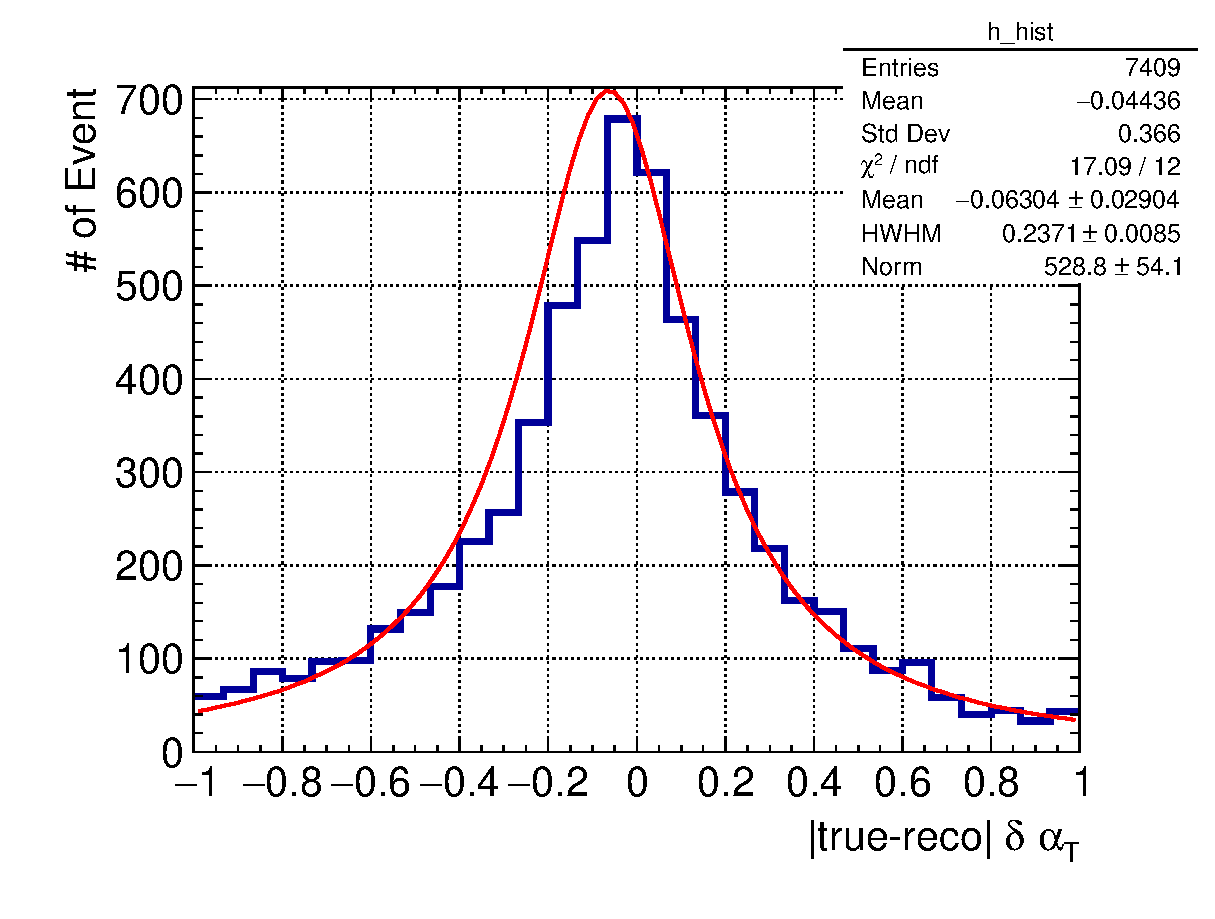
\includegraphics[width=\textwidth]{fig/dalphat_rat_hist_al13.eps}
                \caption{$\dat$ resolution before ESC selection.}
                \label{fig:dat-res-bfESC}
           \end{subfigure}
           \begin{subfigure}{0.45\textwidth}
                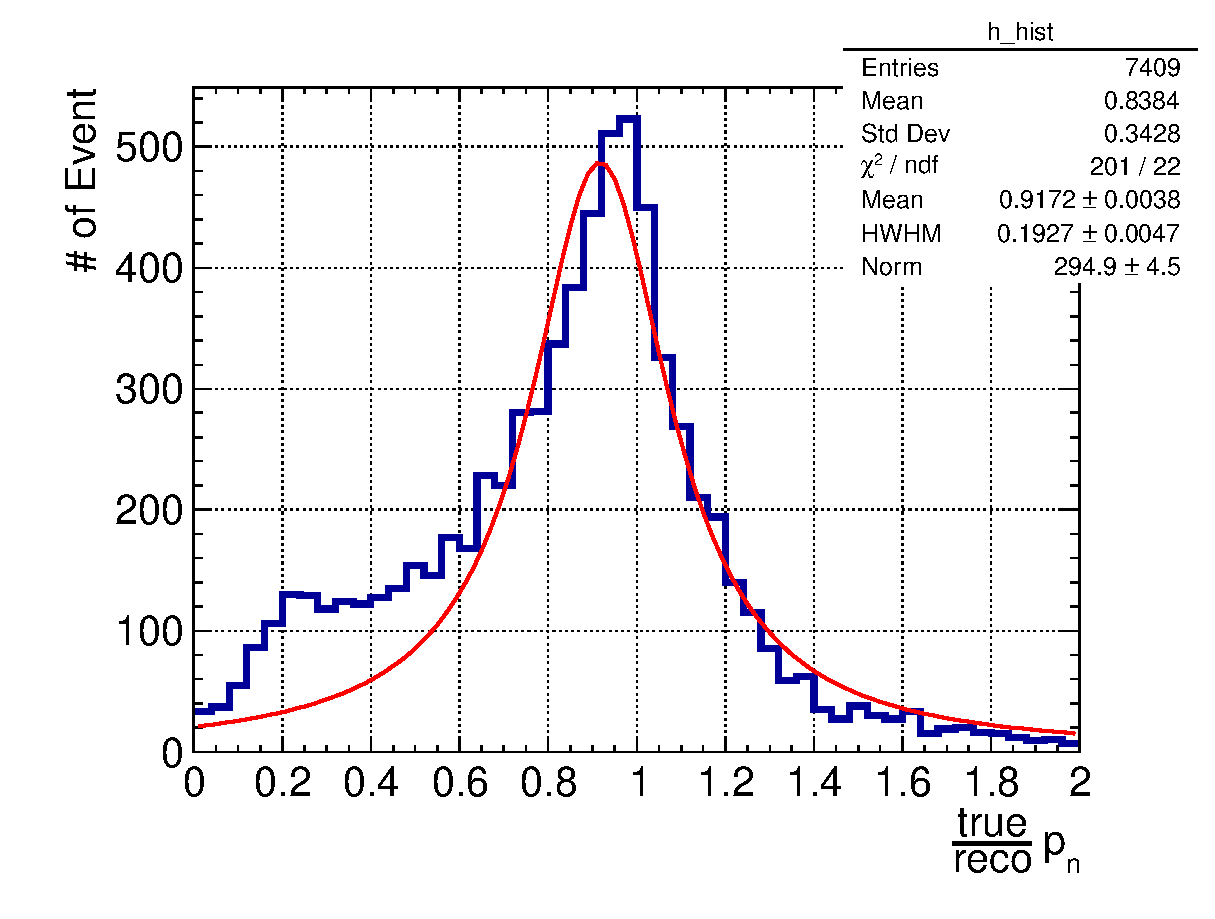
\includegraphics[width=\textwidth]{fig/pn_rat_hist_al13.eps}
                \caption{$\pn$ resolution before ESC selection.}
                \label{fig:pn-res-bfESC}
           \end{subfigure}
           \\
            \begin{subfigure}{0.45\textwidth}
                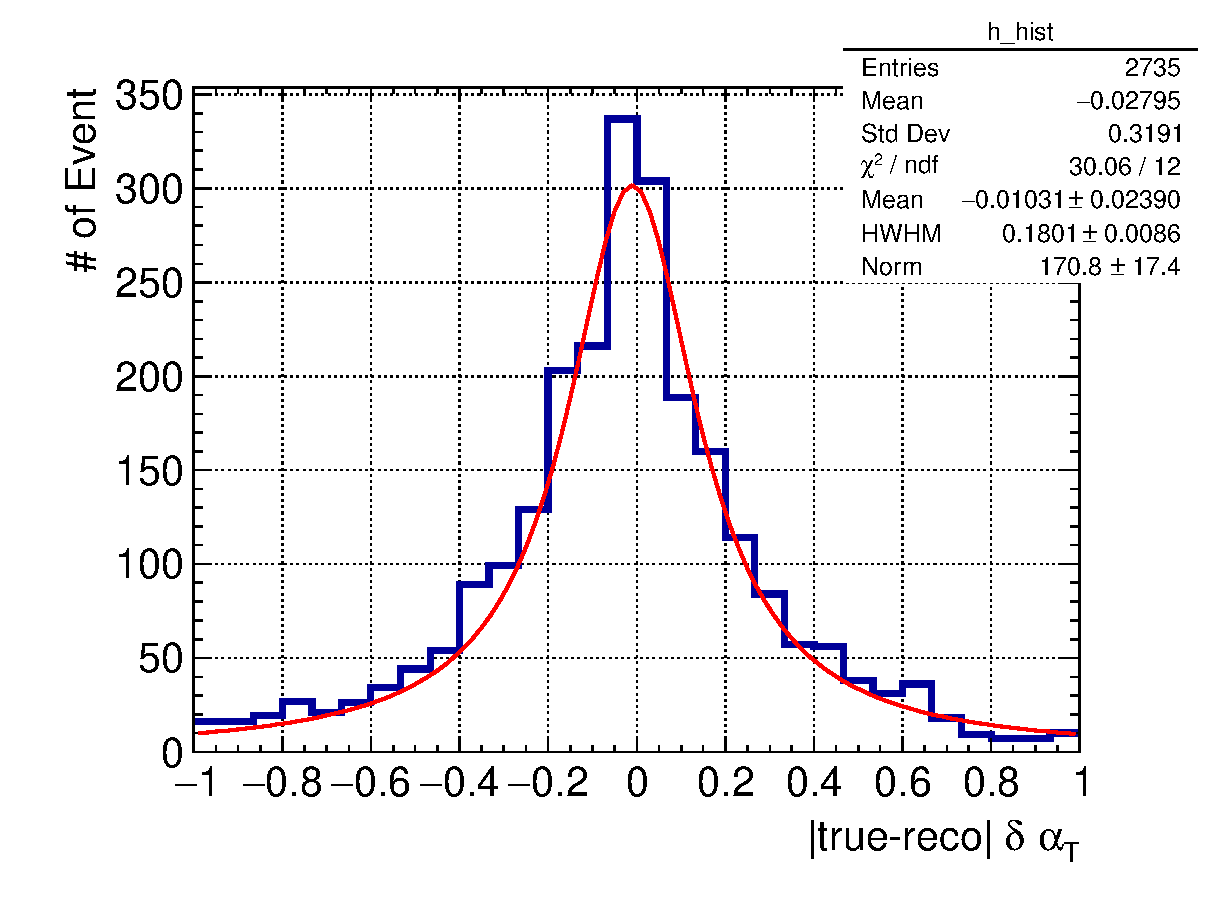
\includegraphics[width=\textwidth]{fig/dalphat_rat_hist_al14.eps}
                \caption{$\dat$ resolution after ESC selection.}
                \label{fig:dat-res-afESC}
           \end{subfigure}
           \begin{subfigure}{0.45\textwidth}
                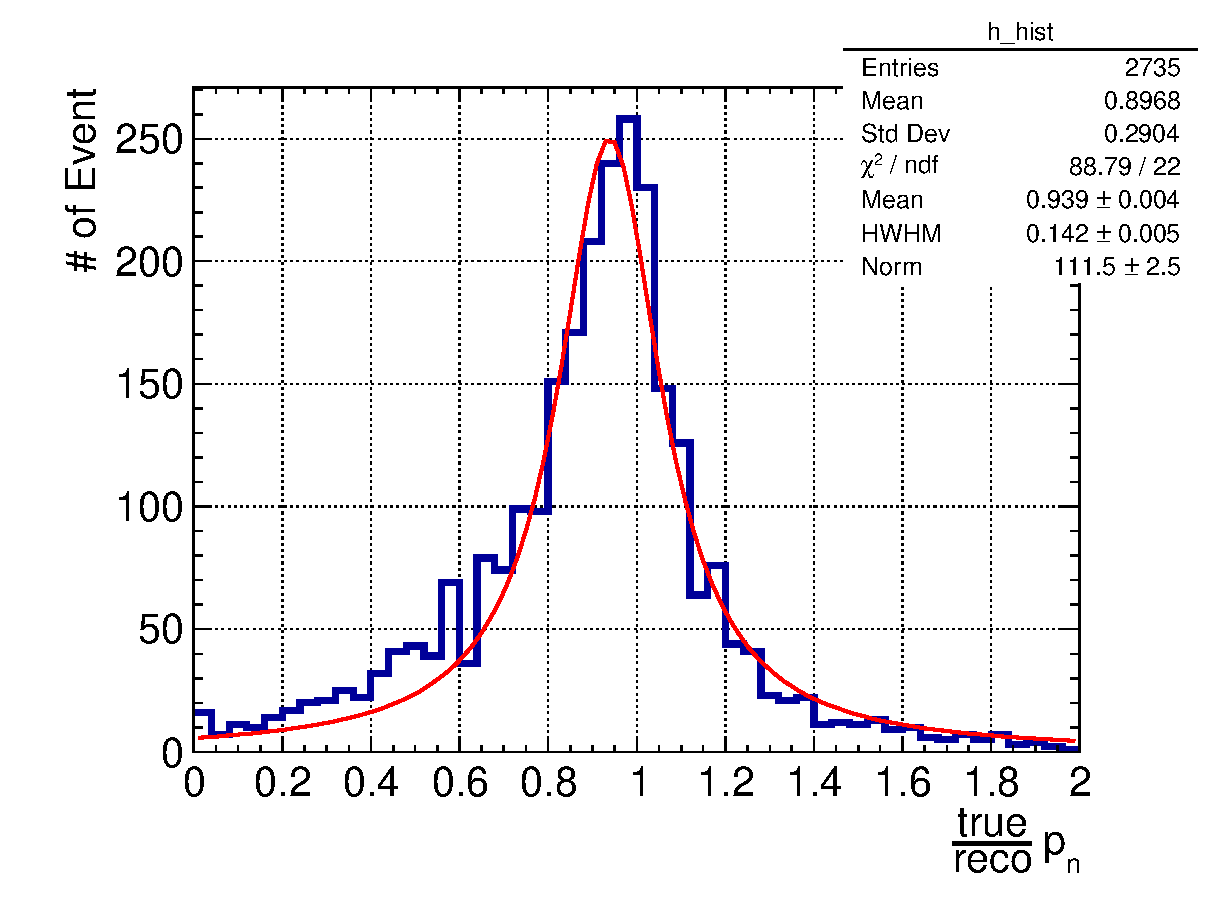
\includegraphics[width=\textwidth]{fig/pn_rat_hist_al14.eps}
                \caption{$\pn$ resolution after ESC selection.}
                \label{fig:pn-res-afESC}
           \end{subfigure}
           \\
            \begin{subfigure}{0.45\textwidth}
                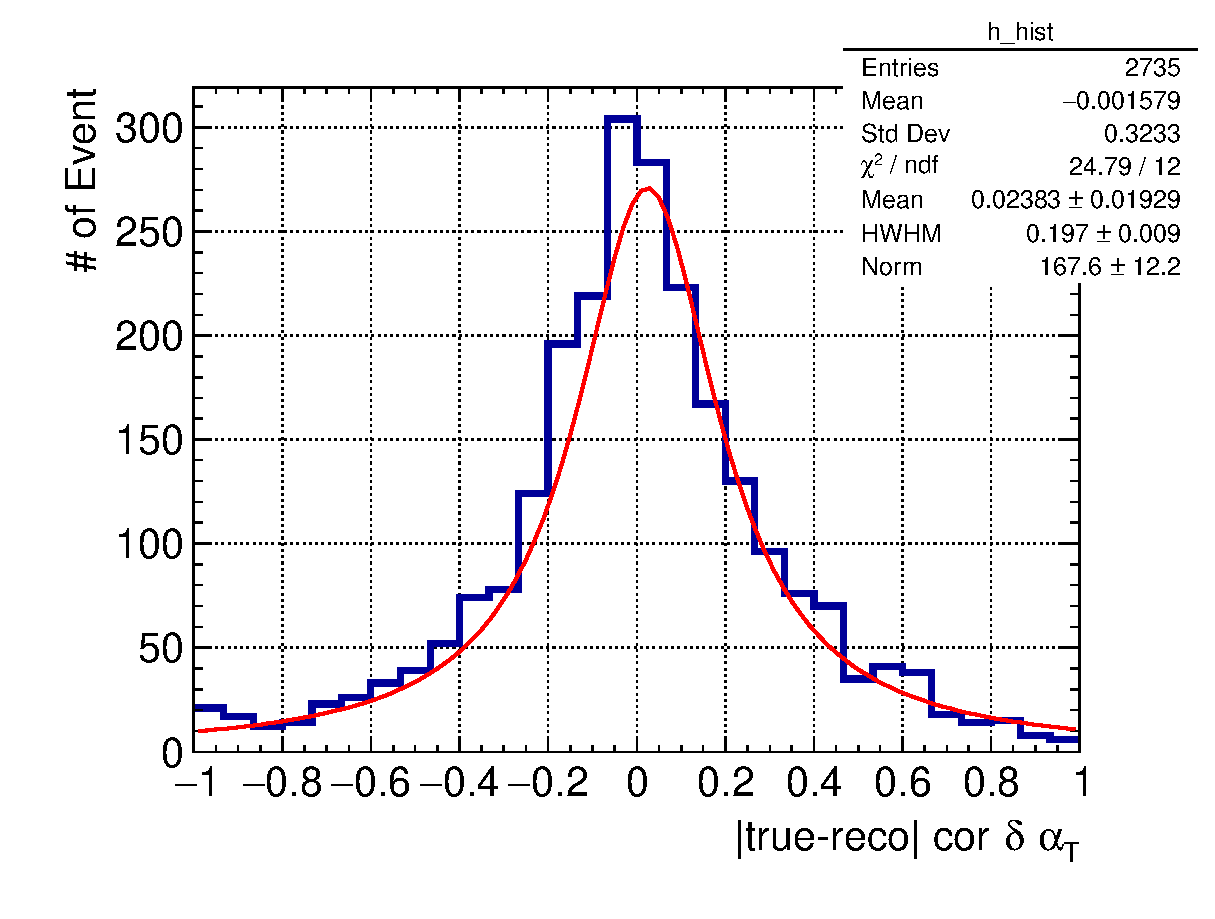
\includegraphics[width=\textwidth]{fig/cor_dalphat_rat_hist_al14.eps}
                \caption{$\dat$ resolution after $\pmut$ correction.}
                \label{fig:0pi-cordat}
           \end{subfigure}
           \begin{subfigure}{0.45\textwidth}
                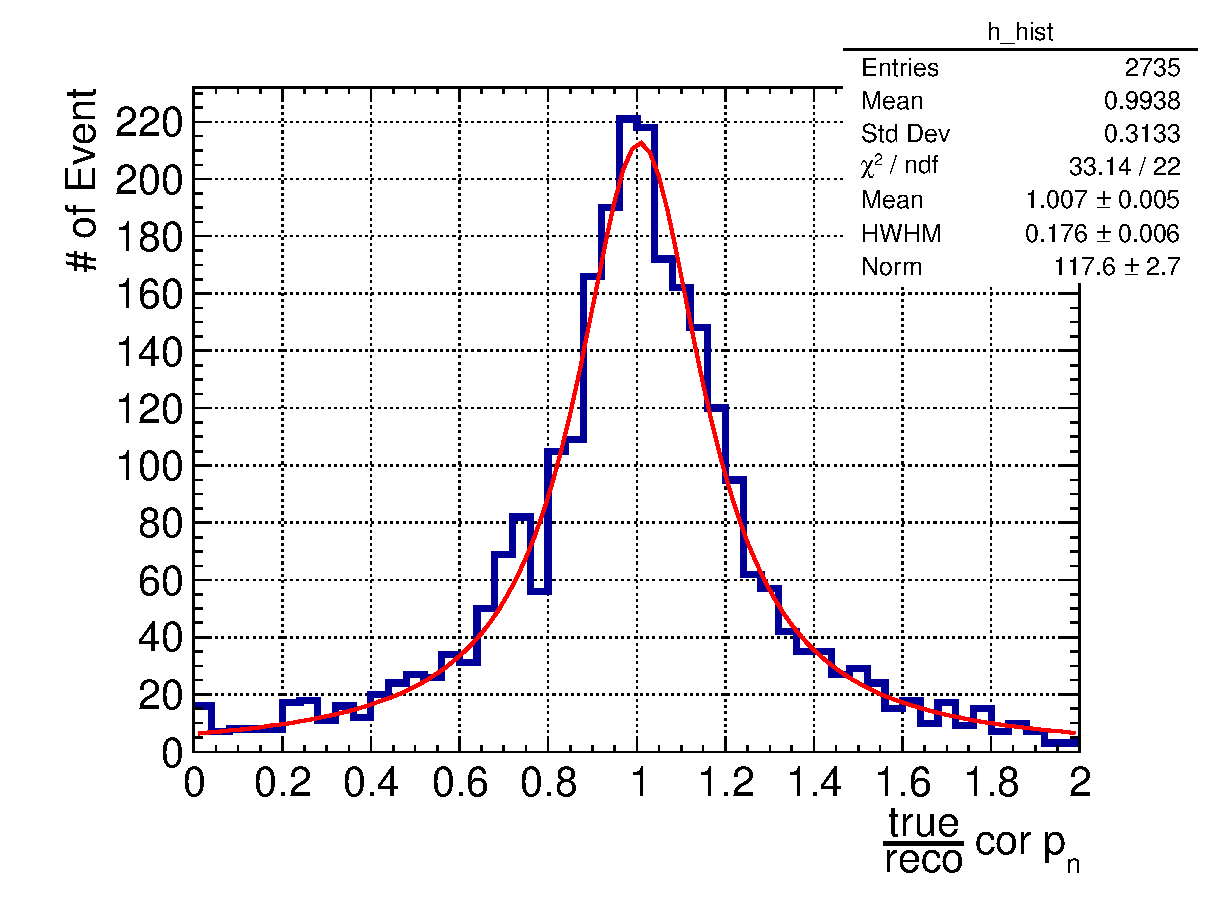
\includegraphics[width=\textwidth]{fig/cor_pn_rat_hist_al14.eps}
                \caption{$\pn$ resolution after $\pmut$ correction.}
                \label{fig:0pi-corpn}
           \end{subfigure}
           \caption{TKI reconstruction results.}
           \label{fig:tki-res-bfafESC}
        \end{figure}

        With the ESC selection, the resolution of $\dat$ and $\pn$ has improved considerably from $0.23$ to $0.18~\textrm{rad}$ and from $19.3\%$ to $14.2\%$ respectively. Moreover, the fitted bias has decreased from $-0.06$ to $-0.01~\textrm{rad}$ and from $1-0.917=0.083$ to $1-0.939=0.061$ for $\dat$ and $\pn$ respectively.  

        As pointed out in Ref.~\cite{Lu:2016mjf}, the ESC selection might lead to a bias in the particle transverse momentum. 
        Such transverse bias would have to be checked after the ESC selection and, if any, corrected for better TKI measurement. 
        The results of the bias check are summarised in Fig.~\ref{fig:0piptbiascheck}. 
        There is no transverse bias for proton as shown in Fig.~\ref{fig:0pi-prpt-bias}, while there is a clear bias in muon $\pt$ for $0.5<\pmut<1.1~(\gevc)$. 
        It is further checked that this bias is not due to a bias in the angle reconstruction, as shown in Fig.~\ref{fig:0pi-mutheta-bias}.
        Thus, a correction is directly applied to $\pmut$ within the specified range, and the corrected $\pmut$ is shown in Fig.~\ref{fig:cormupt}.

       \begin{figure}[!htb]
           \centering
           \begin{subfigure}{0.3\textwidth}
                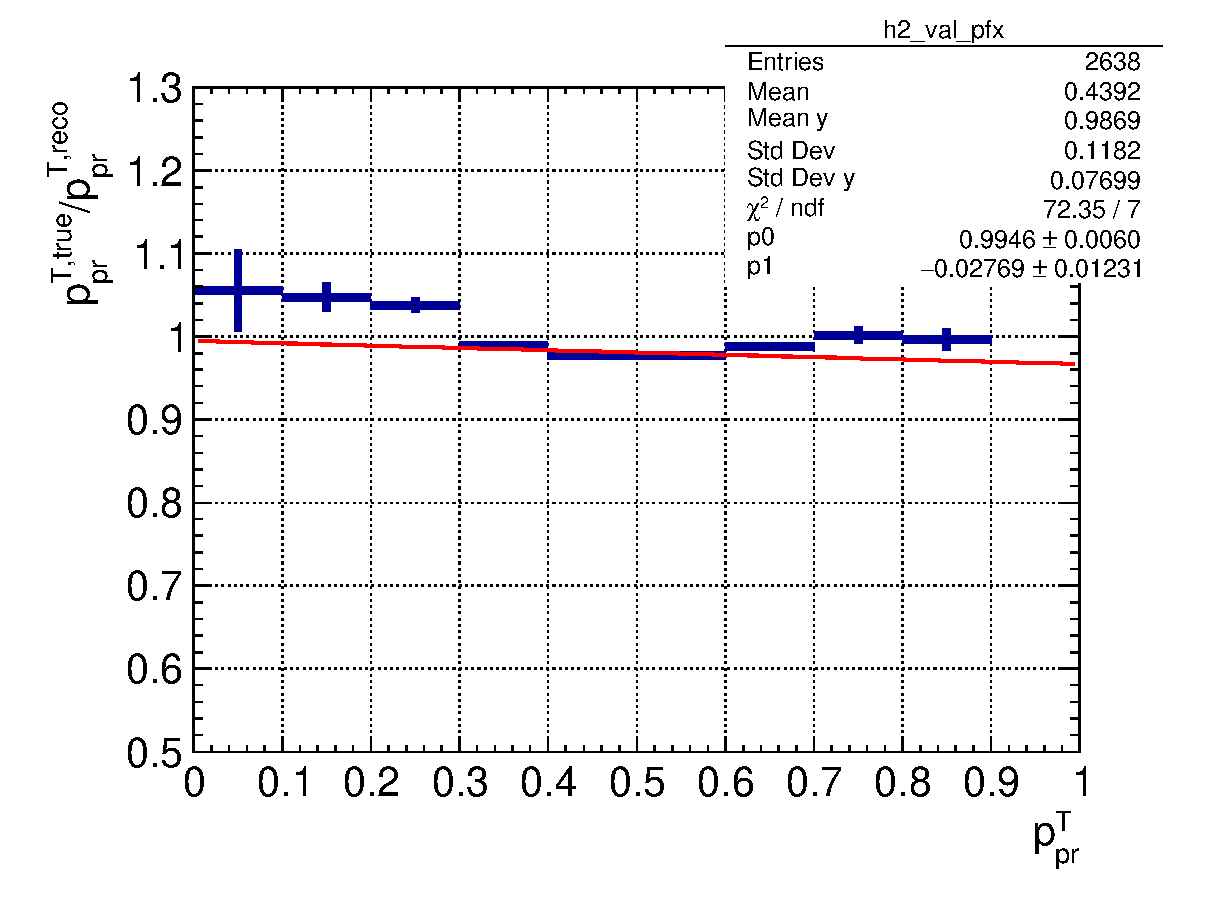
\includegraphics[width=\textwidth]{fig/pr_pt_vs_pr_pt_bias_hist2d_al14.eps}
                \caption{Proton transverse bias.}
                \label{fig:0pi-prpt-bias}
           \end{subfigure}
           \begin{subfigure}{0.3\textwidth}
                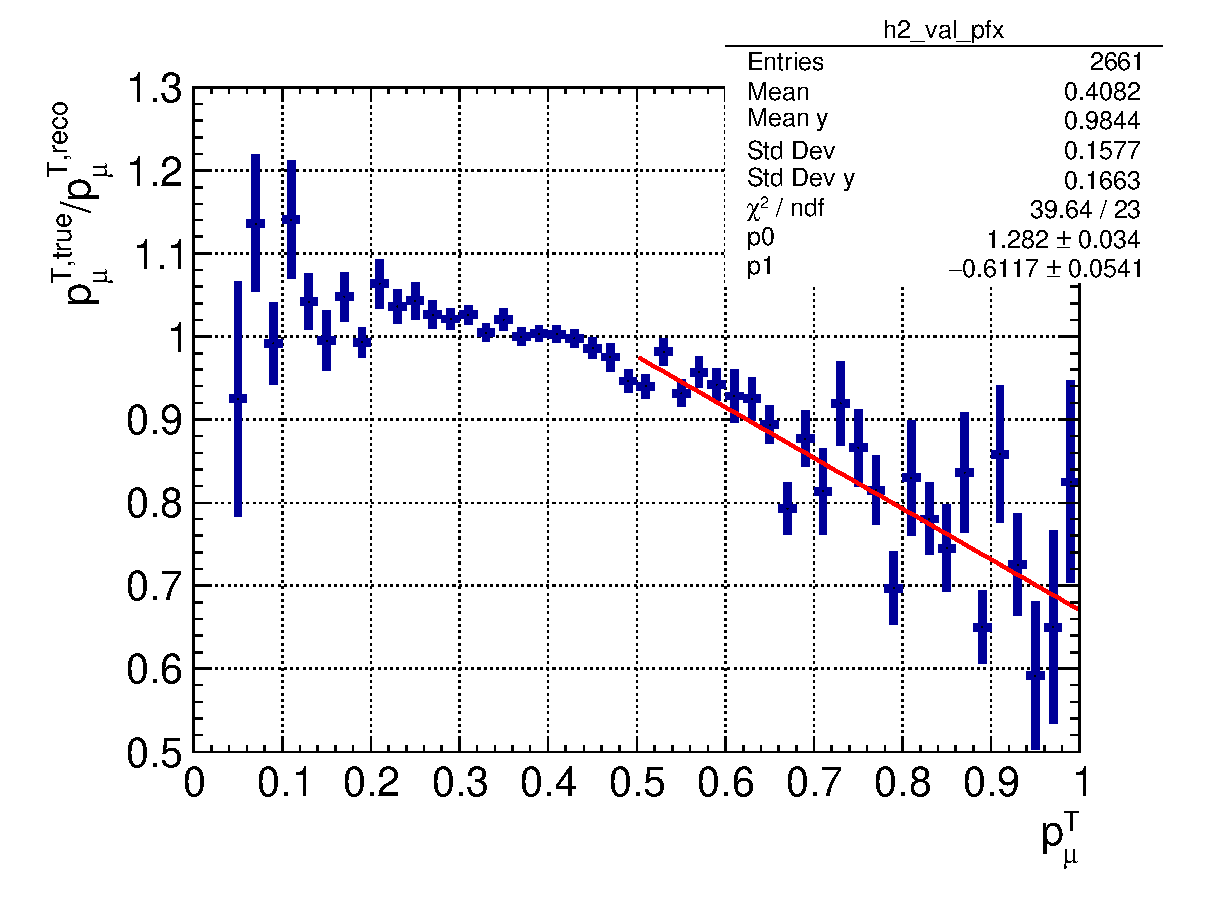
\includegraphics[width=\textwidth]{fig/mu_pt_vs_mu_pt_bias_hist2d_al14.eps}
                \caption{Muon transverse bias.}
                \label{fig:0pi-mupt-bias}
           \end{subfigure}
           \begin{subfigure}{0.3\textwidth}
                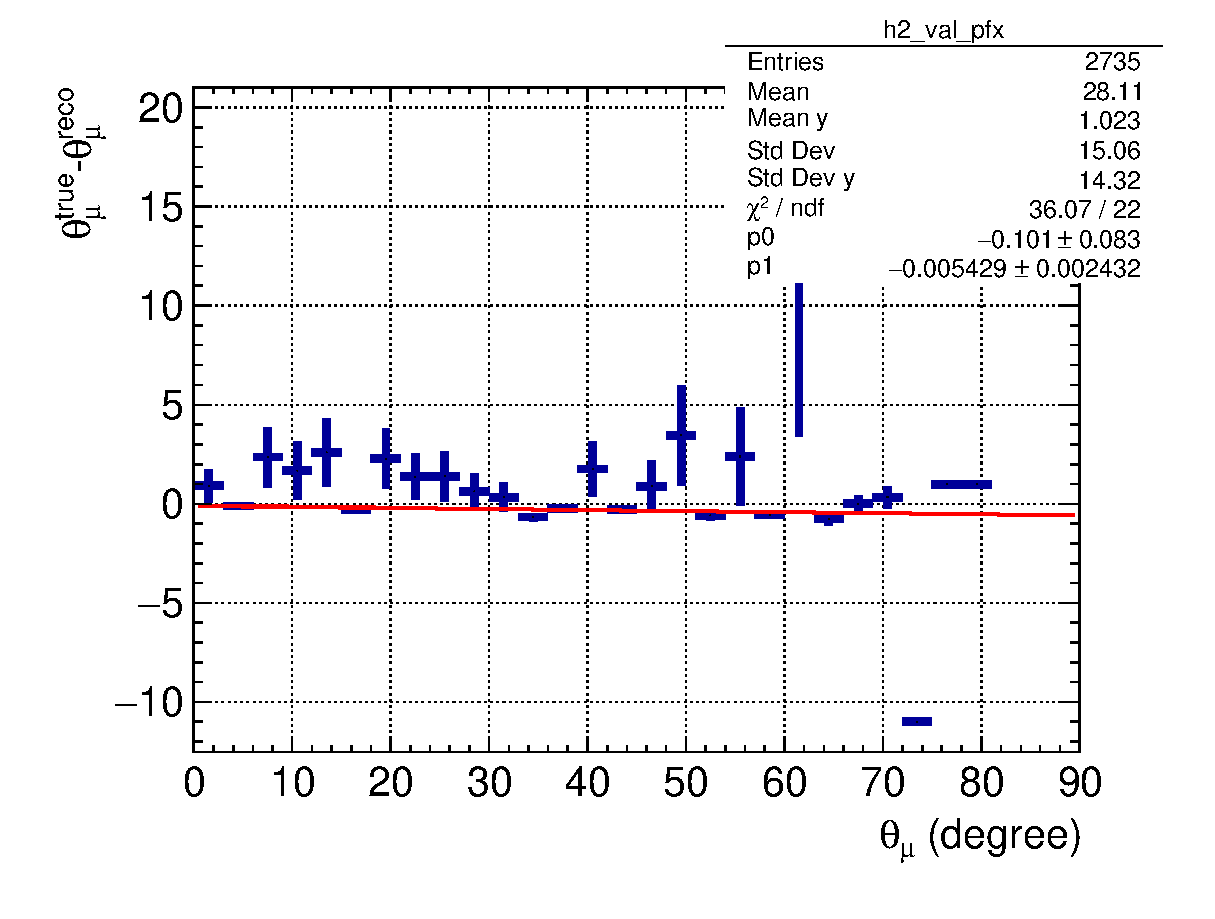
\includegraphics[width=\textwidth]{fig/theta_mu_vs_theta_mu_res_hist2d_al14.eps}
                \caption{Muon theta bias.}
                \label{fig:0pi-mutheta-bias}
           \end{subfigure}
           \caption{Transverse bias check after ESC selection.}
           \label{fig:0piptbiascheck}
        \end{figure}
            
        \begin{figure}[!htb] 	
            \centering 		
            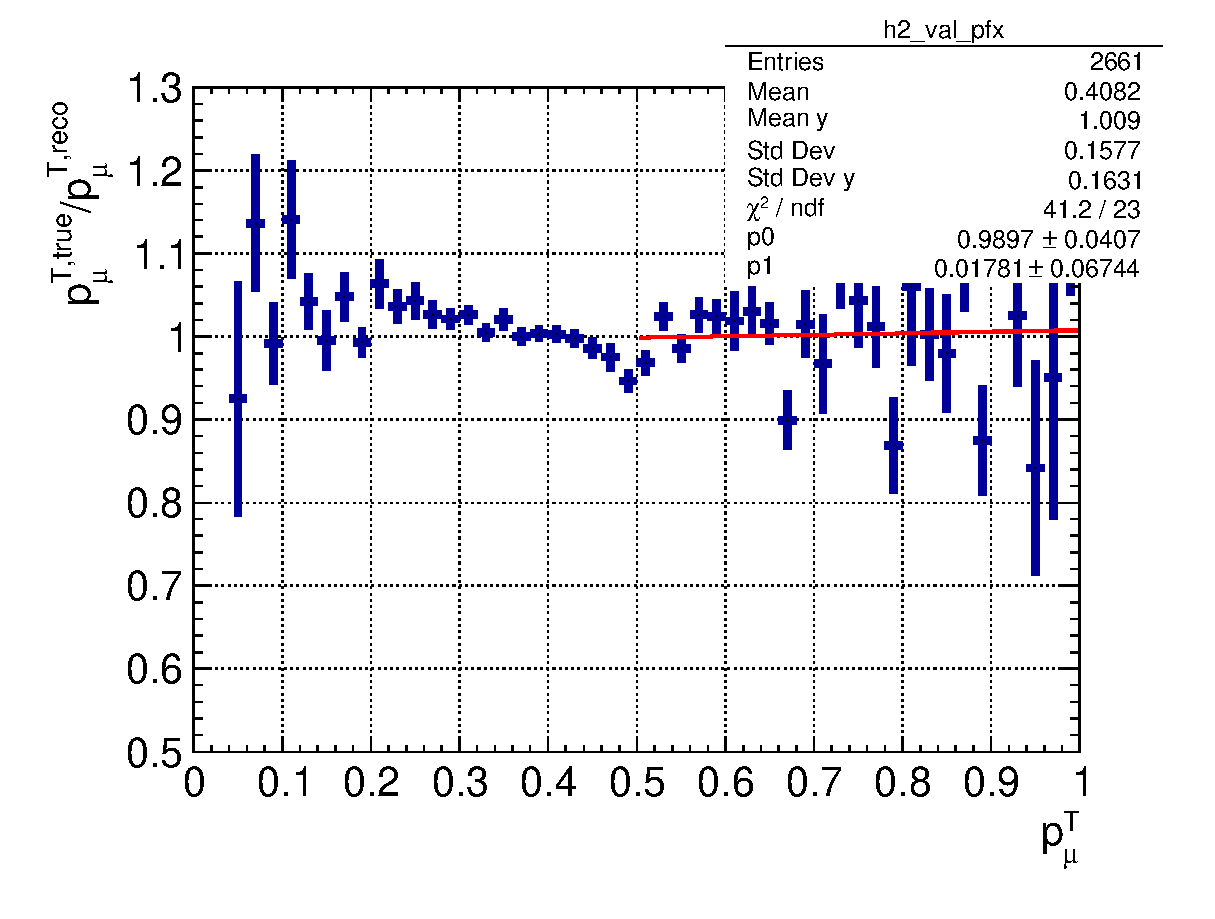
\includegraphics[width=0.35\textwidth]{fig/mu_pt_vs_cor_mu_pt_bias_hist2d_al14.eps}
            \caption{\label{fig:cormupt} Corrected $\pmut$.} 
        \end{figure}

        The impact of the $\pmut$ correction on the TKI variables are shown in Fig.~\ref{fig:0pi-cordat} and Fig.~\ref{fig:0pi-corpn}. The resolutions remain similar, while the bias in $\pn$ has significantly reduced from $6.1\%$ to $0.7\%$.

    \subsection{\label{sec:1pi-tki} TKI in $\numuccopiop$ selection}

    As I have the $\numuccopi$ selection along with the pion trackless reconstruction, it is straightforward to select a $\numuccopiop$ sample by adding an extra step of requiring exactly one SFGD contained proton that passes the ESC selection. 
    The $\pt$ biases are checked for all three particles and no biases are observed. Hence, the final TKI reconstruction results are given in Fig.~\ref{fig:1pi-tki-res}. Both $\dat$ and $\pn$ have minimal fitted bias, $-0.02~\textrm{rad}$ for $\dat$ and about $2\%$ for $\pn$. While the $\dat$ has a slightly worse resolution, $0.24~\textrm{rad}$, than that in $\numucczpiop$, $\pn$ has a better resolution, $12\%$. 
    
   \begin{figure}[!htb] 
       \centering
       \begin{subfigure}{0.45\textwidth}
            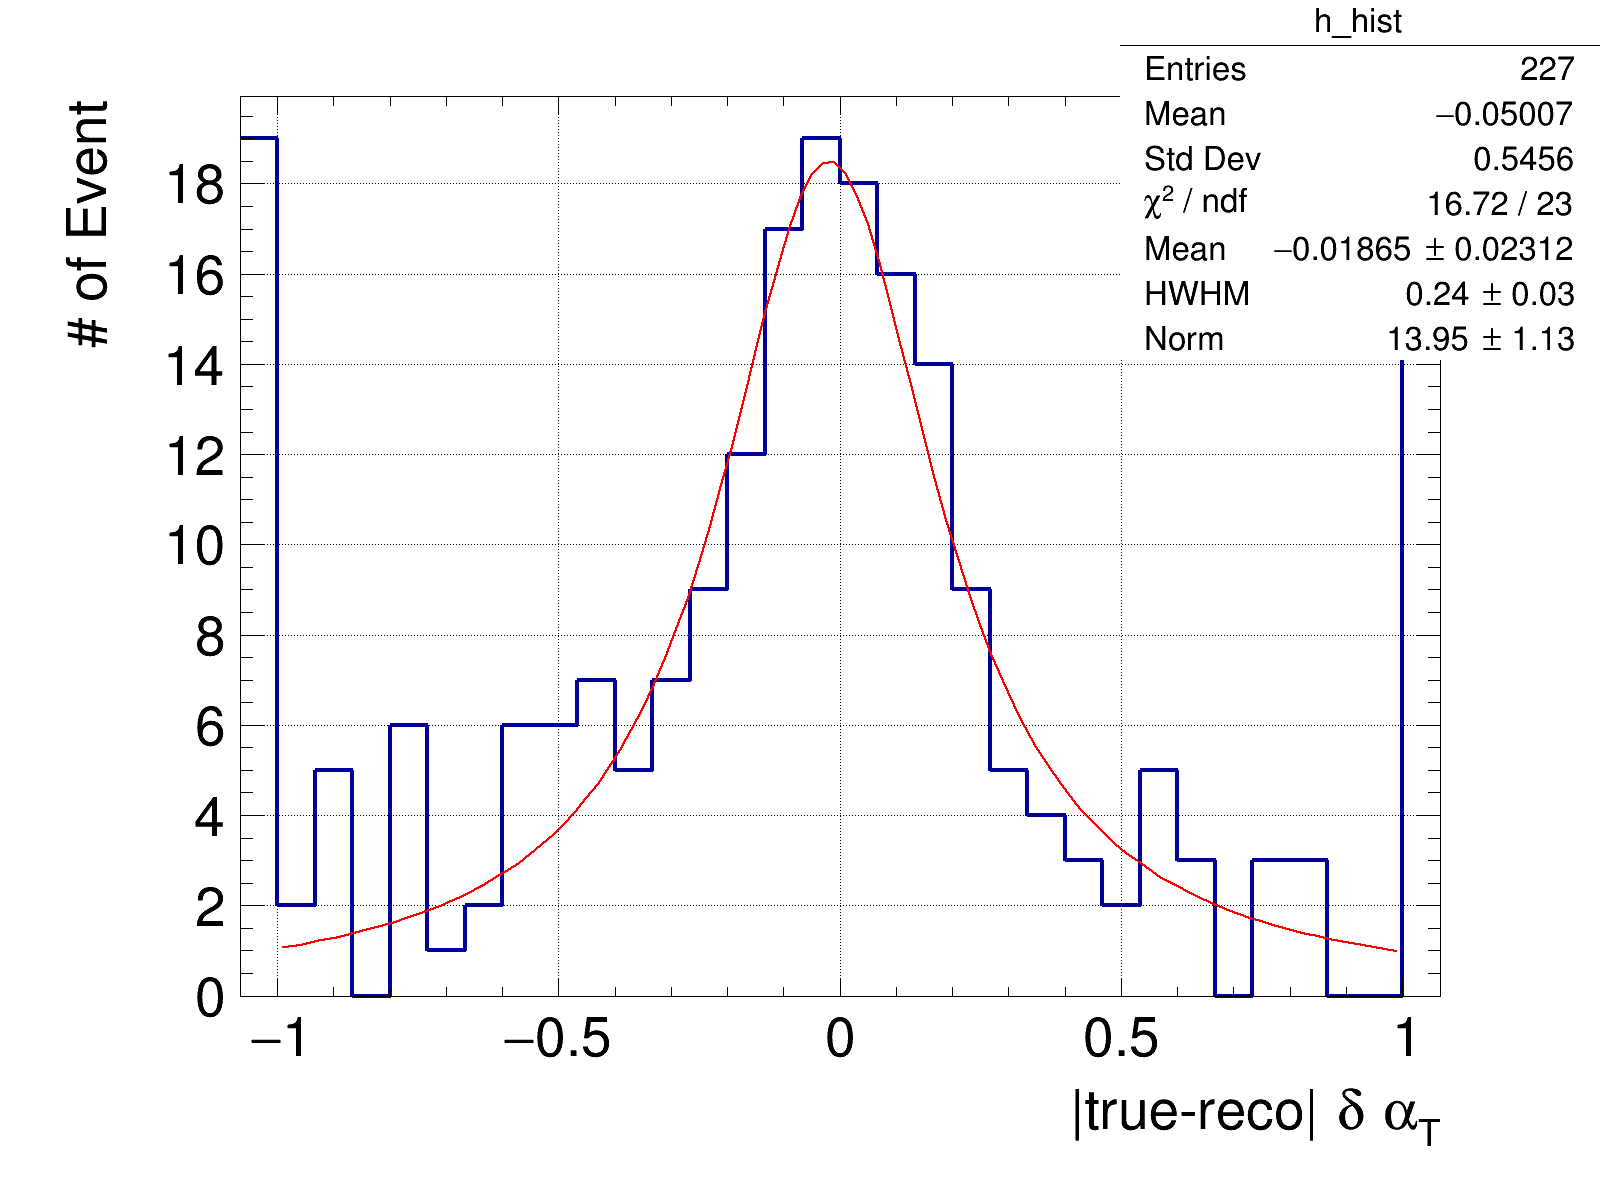
\includegraphics[width=\textwidth]{fig/SFGpTPCmu_dalphat_rat_hist_al14.png}
            \caption{$\dat$ resolution.}
            \label{fig:1pi-dat-res}
       \end{subfigure}
       \begin{subfigure}{0.45\textwidth}
            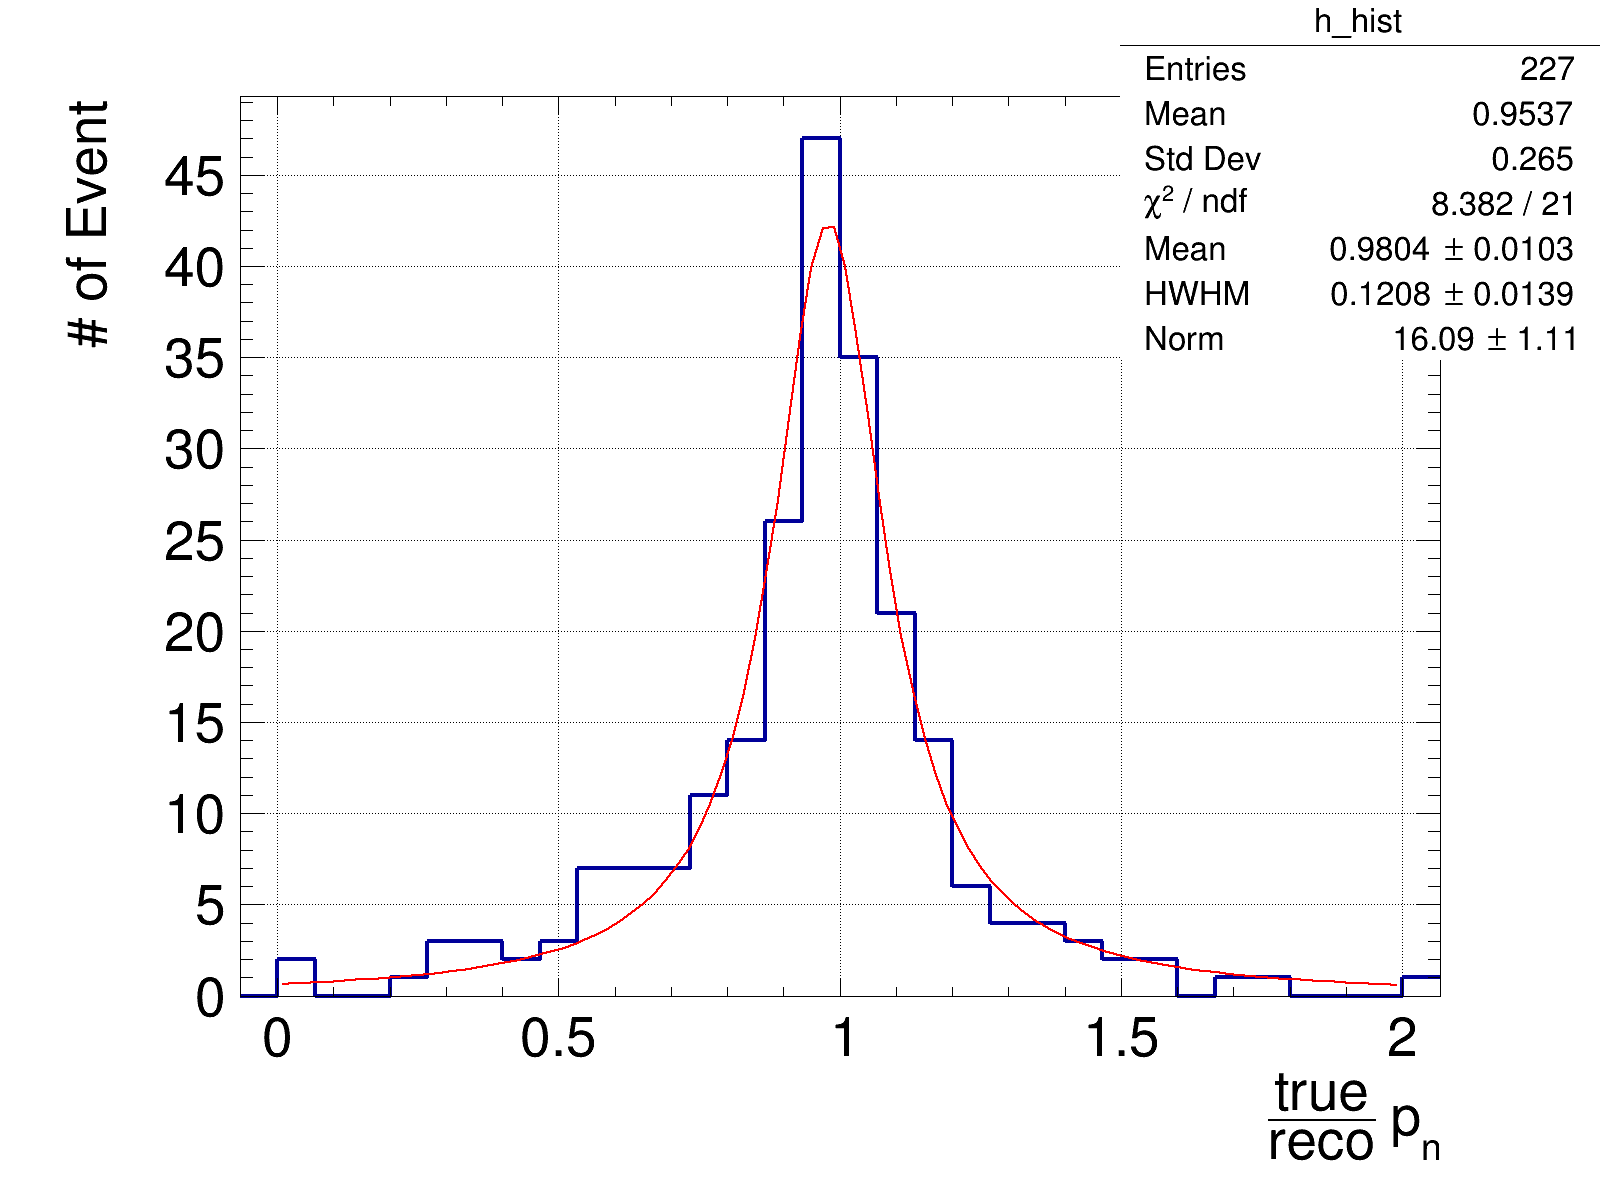
\includegraphics[width=\textwidth]{fig/SFGpTPCmu_pn_rat_hist_al14.png}
            \caption{$\pn$ resolution.}
            \label{fig:1pi-pn-res}
       \end{subfigure}
       \caption{TKI reconstruction results.}
       \label{fig:1pi-tki-res}
    \end{figure}

    In additional to the single transverse variables presented above, the $\numuccopiop$ sample can also be used to measure the double transverse variable, $\dptt$, the net momentum transverse to both the neutrino momentum and the muon momentum,
    Without FSI, $\dptt$ should be $0$. This special property can be exploited to select $\nu$-H events amidst $\nu$-C events as suggested in Ref.~\cite{dpttpaper}. 
    Hence, the main figure of merit for $\dptt$ measurement is the width of its distribution for $\nu$-H events, where the hydrogen events are picked by an additional check on the MC truth information.
    As shown in Fig.~\ref{fig:dptt-hist}, the fitted half width is about $12~\mevc$, which is significantly improved compared to $21~\mevc$, the pre-upgrade ND280 result \cite{dpttpaper}.

    \begin{figure}[!htb] 
        \centering 		
        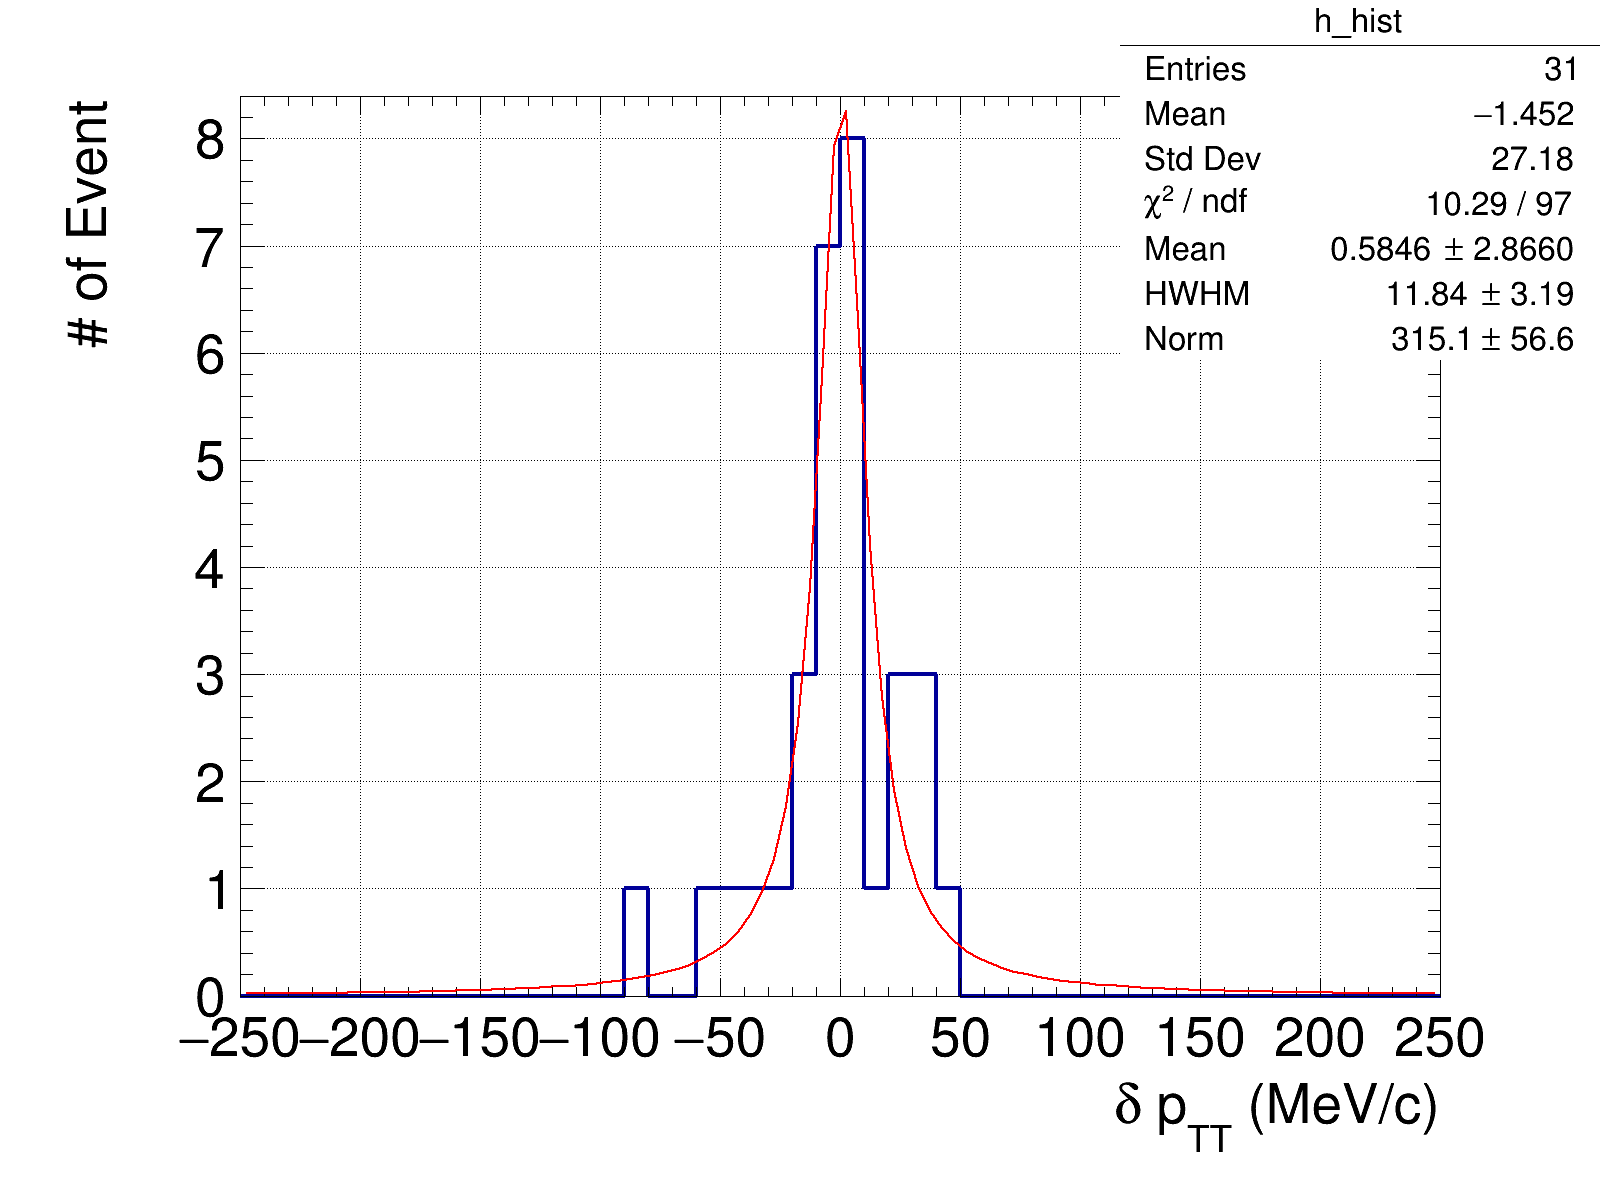
\includegraphics[width=0.35\textwidth]{fig/SFGpTPCmu_dptt_hist_al15_H_bin100_range500_Lfit.png}
        \caption{\label{fig:dptt-hist} $\dptt$ distribution for $\nu$-H events.} 
    \end{figure}


\section{Tuning}

    The potential improvement in reconstruction at the ND upgrade is promising, but the actual effect on measurement can only be evaluated after sufficient data are collected. 
    In preparation for maximising the physical impact of the future measurement, I embarked on a tuning project using the \genie Comparisons framework, which explores the potential of improving simulation models using measurement and will be immediately useful when the upgrade measurement is available. 
    
    As I am most familiar with the TKI measurements and there has not been a global tune using both data with and without pions in the final states, this tuning project has also filled in this gap nicely by looking at $4$ TKI data sets: T2K $0\pi$~\cite{T2K:2018rnz}, T2K $\pi^+$~\cite{T2K:2021naz}, MINERvA $0\pi$~\cite{MINERvA:2018hba, MINERvA:2019ope}, and MINERvA $\pi^0$~\cite{MINERvA:2020anu} measurements. 
    The two $0\pi$ data sets are both based on $\numucczpinp$ selections, while \ttkpip requires exactly $1$ additional $\pip$ and \minpiz requires at least $1$ additional $\piz$. Each data set has a slightly different kinematic cuts summarised in Table~\ref{tab:data-sets-phase-space-cut}.

        \begin{table}[!htb]
        \centering
        \begin{tabular}{cc}
        \hline
        \hline
        Variables & Cuts ($p$ in $\gevc$) \\
        \hline
        \multicolumn{2}{c}{\ttkzpi~\cite{T2K:2018rnz}} \\
        \hline
        $\vecpmu$    &  $0.25 < p_\mu $, $\cos\theta_\mu>-0.6$   \\
        $\vecpp$     & $0.45< p_\text{p} <1.0$ , $\cos\theta_\text{p}>0.4$     \\
        \hline
        \multicolumn{2}{c}{\ttkpip~\cite{T2K:2021naz}} \\
        \hline
        $\vecpmu$    & $0.25 < p_\mu < 7$ , $\theta_\mu < 70^\degree$  \\
        $\vecpp$     & $0.45 < p_\text{p} <1.2$  ,  $\theta_\text{p} < 70^\degree$   \\
        $\vecppi$    & $0.15 < p_\pi <  1.2$, $\theta_\pi < 70^\degree$ \\
        \hline
        \multicolumn{2}{c}{\minzpi~\cite{MINERvA:2018hba, MINERvA:2019ope}} \\
        \hline
        $\vecpmu$     & $1.5< p_\mu < 10$ , $\theta_\mu < 20^\degree $  \\
        $\vecpp$      & $0.45< p_\text{p} <1.2$  , $\theta_\text{p} < 70^\degree$    \\
        \hline
        \multicolumn{2}{c}{\minpiz~\cite{MINERvA:2020anu}} \\
        \hline
        $\vecpmu$   & $1.5< p_\mu < 20$ , $\theta_\mu < 25^\degree$  \\
        $\vecpp$    & $0.45< p_\text{p} $                      \\
        \hline
        \hline
        \end{tabular}
        % \end{ruledtabular}
        \caption{\label{tab:data-sets-phase-space-cut}
        Kinematic cuts for the samples of the TKI measurements.
        }
    \end{table}

    Since the TKI measurements are most sensitive to the initial state and FSI, this work investigates a partial tune of these two processes to derive an effective model capable of describing well both neutrino-nuclear pion production and pionless production. 
    The nominal \genie configuration used is the \newtune ~ (\gZero ~ for short), which captures previous tuning efforts in Ref.~\cite{GENIE:2021zuu} and implements more advanced models. The detailed model specification of this configuration is given in Table~\ref{tab:default-gen-list}.

    \begin{table}[!htb]
        \centering
        \begin{tabular}{p{4cm}c}
        \hline
        \hline
        \textrm{Simulation component} & \textrm{Model} \\
        \hline
        \textrm{Nuclear state}              & \sfcfg~\cite{sfcfg-talk,sfcfg-GitHubCommit,GENIE:2021npt} \\ 
        \textrm{QE}               & Valencia~\cite{Nieves:2004wx} \\
        \textrm{2p2h}               & SuSAv2~\cite{Gonzalez-Jimenez:2014eqa} \\
        \textrm{QE $\Delta S=1$}           & Pais~\cite{Pais:1971er} \\
        \textrm{QE $\Delta C=1$}                  & Kovalenko~\cite{Kovalenko:1990zi} \\
        \textrm{Resonance (RES)}                        & Berger-Sehgal~\cite{Berger:2007rq}\\
        Shallow/Deep inelastic \par scattering (SIS/DIS)                    & Bodek-Yang~\cite{Bodek:2002vp}\\
        \textrm{DIS $\Delta C=1$}           & Aivazis-Tung-Olness~\cite{Aivazis:1991fy}\\
        \textrm{Coherent $\pi$ production}  & Berger-Sehgal~\cite{Berger:2008xs}\\
        \hline
        \textrm{Hadronization}              & AGKY~\cite{Yang:2009zx}\\
        \textrm{FSI}                        & INTRANUKE hA~\cite{Andreopoulos:2015wxa}\\
        \hline
        \hline
        \end{tabular}
        \caption{\label{tab:default-gen-list} Model components of \gZero. Processes with non-trivial $\Delta S$ and $\Delta C$ are those with strangeness and charm production, respectively.}
    \end{table}



    \subsubsection{Tuning Implementation}
    
        This study adopts the tuning procedure outlined in Ref.~\cite{GENIE:2022qrc}, utilising $N_{\textrm{par}}$ model parameters. 
        The objective is to identify the optimal set of parameter values that minimise the $\chi^2$ between model predictions and data. 
        Given the high dimensionality of the parameter space, a brute-force grid scan is impractical. 
        Therefore, a sufficient number of points is first randomly picked. 
        Each point is then used to run a full event generation. 
        The simulation prediction for each data bin is parameterised using Professor~\cite{Buckley:2009bj} with a polynomial of the model parameters of a chosen order, $N_{\textrm{ord}}$.
        The $\chi^2$ minimisation is run between this polynomial estimation and data. 
        Since the parameterisations are polynomials, the minimisation is fast. 

        The two key ingredients of the tuning procedure are the data observables used and the model parameters to be tuned. 
        The full set of available data is given in Table~\ref{tab:data-sets}. 
        To identify the most sensitive variables, various combinations were used in tuning. 
        The observables that are not used in a combination for tuning will still calculate a $\chi^2$ for validation, since a physical model should describe all these observables well simultaneously. 
        \begin{table}[!htb]
            \centering
            \begin{tabular}{ccccc}

            \hline
            \hline
            Observables & No. of  bins & \texttt{Combi-Superset}  & \texttt{Combi-Best-}\allpar & \texttt{Combi-Best-}\redpar\\
            \hline
            \multicolumn{5}{c}{\ttkzpi} \\
            \hline
               $\dat$            & $8$                & $\tick$     &  & $\tick$  \\ 
               $\dpt$            & $8$                & $\tick$     & $\tick$  & $\tick$ \\ 
               $\dphit$          & $8$                & $\tick$     &  &  \\      
            \hline
            \multicolumn{5}{c}{\ttkpip} \\
            \hline
              $\dat$            & $3$                & $\tick$      &  & $\tick$  \\
              $\pn$             & $4$                & $\tick$      & $\tick$  & $\tick$ \\ 
              $\dptt$           & $5$                & $\tick$      &  & $\tick$  \\ 
            \hline
            \multicolumn{5}{c}{\minzpi} \\
            \hline  
              $\dat$            & $12$               & $\tick$      & & $\tick$  \\ 
              $\pn$             & $24$               & $\tick$      & $\tick$  & $\tick$ \\
              $\dpt$            & $24$               & $\tick$      & $\tick$ &  \\     
              $\dphit$          & $23$               & $\tick$      &  &  \\     
              $\pp$             & $25$               &      &  &  \\     
              $\thetap$         & $26$               &      &  &  \\     
              $\dptx$           & $32$               &      &  &  \\  
              $\dpty$           & $33$               &      &  & \\     
            \hline
            \multicolumn{5}{c}{\minpiz} \\
            \hline
              $\dat$            & $9$               & $\tick$      & & $\tick$      \\  
              $\pn$             & $12$               & $\tick$     & $\tick$  & $\tick$ \\ 
              $\dptt$           & $13$               & $\tick$     &  & $\tick$  \\
            \hline
            \hline
            \end{tabular}
            \caption{\label{tab:data-sets}
        	Observables of the TKI measurements and their binning. Those with ``$\tick$''s are used for tuning, while those without  are for the respective validation. See Table~\ref{tab:hALFG-para} for definitions of \cbRedPar and \cbAllPar.
            }
        \end{table}

         In this project, only the currently tunable parameters within the Spectral-Function-like Correlated Fermi Gas (\sfcfg) and the FSI model, hA, models are explored, leading to a total of $14$ parameters (collectively referred to as the \allpar set) as detailed in Table~\ref{tab:hALFG-para}. 
         Nominal values and associated uncertainties for the hA model are taken from Table 17.3 in Ref.~\cite{Andreopoulos:2015wxa}. 
         The two most relevant parameters in \sfcfg are $\srcfr$, representing the fraction of the high-momentum tail from short-range correlations (SRC), notably above the Fermi surface, and $\nurmec$, marking the commencement of the nuclear removal energy distribution for carbon. 
         A larger $\srcfr$ indicates the presence of more energetic initial nucleons, while an increased $\nurmec$ implies that greater energy is necessary to liberate a nucleon from the carbon nucleus, so the product particles will possess lower energy. 
         As for the hA model, there are two main categories of parameters. One is the MFP scaling factors for pions and nucleons ($\cpimfp$, $\pizmfp$,  and $\nmfp$) detailed in Table~\ref{tab:hALFG-para}, the other is the relative scaling factors for $4$ rescattering types, charge exchange (CEX), inelastic scattering (INEL), absorption (ABS), and pion production (PIPD), e.g. $\picex$.
         
        \begin{table}[!htb]
        \centering
        % \begin{tabular}{cp{1.5cm}p{1.5cm}p{1.2cm}p{1.2cm}}
        \begin{tabular}{ccccc}
        \hline
        \hline
        \textrm{Parameter} & \textrm{Nominal} (\gZero)     & \textrm{Range In Tuning} & \allpar (\gT)  & \redpar (\gC) \\ 
        \hline
        \multicolumn{5}{c}{\sfcfg} \\
        \hline
        \textrm{$\srcfr$} & 0.12 & (0.0, 0.5)  & \tick & \tick\\
        \textrm{$\nurmec$} & 0.01 & (0.0, 0.2) & \tick & \\
        \hline
        \multicolumn{5}{c}{hA} \\
        \hline
        \textrm{$\cpimfp$} & $1.0\pm0.2$ & (0.0, 3.0) & \tick & \\
        \textrm{$\pizmfp$} & $1.0\pm0.2$ & (0.0, 3.0) & \tick & \tick\\
        \textrm{$\nmfp$} & $1.0\pm0.2$ & (0.0, 3.0) & \tick &\\
        \hline
        \textrm{$\picex$} &  $1.0\pm0.5$ & (0.0, 3.0) & \tick & \tick \\
        \textrm{$\ncex$} & $1.0\pm0.5$ & (0.0, 3.0)  & \tick & \tick\\
        \hline
        \textrm{$\piinel$} & $1.0\pm0.4$ & (0.0, 3.0) & \tick & \\
        \textrm{$\ninel$} & $1.0\pm0.4$ & (0.0, 3.0)  & \tick &\\
        \hline
        \textrm{$\cpiabs$} & $1.0\pm0.2$ & (0.0, 3.0) & \tick &\\
        \textrm{$\pizabs$} & $1.0\pm0.2$ & (0.0, 3.0) & \tick &\\
        \textrm{$\nabs$} & $1.0\pm0.2$ & (0.0, 3.0)  & \tick & \tick\\
        \hline
        \textrm{$\pipiprod$} & $1.0\pm0.2$ & (0.0, 3.0) & \tick &\\
        \textrm{$\npiprod$} & $1.0\pm0.2$ & (0.0, 3.0)  & \tick & \tick\\
        \hline
        \hline
        \end{tabular}
        \caption{\label{tab:hALFG-para}
        Tunable parameters and their ranges in the  \sfcfg (\textit{uppermost} group) and hA (\textit{lower} groups, uncertainties from Ref.~\cite{Andreopoulos:2015wxa}) models. Parameters to be tuned in the two sets are marked with ``\tick''s. See later text for definitions of \gT and \gC.
        }
    \end{table}

    After determining the set of data observables and model parameters, I then proceed to tuning. During the minimisation step, priors, usually based on systematic uncertainty, can be imposed on each parameter to prevent it from deviating too much from its default value.     
    Firstly, I tuned all combinations of data with the \allpar parameter set. 
    The total $\chi^2$ changes of the tuning output are given by the solid blue bar in Fig.~\ref{fig:allchi}. 
    Surveying the tuned parameters, I observed that for most combinations, certain parameters remained close to their default values, within $1$ $\sigma$ of the imposed prior means, such as $\pipiprod$. 
    This is reasonable since none of the data sets has a significant contribution from PIPD of pions---Removing these parameters from the tuning process does not significantly affect the outcome.
    Therefore, I selected a reduced set comprising only $\srcfr$, $\pizmfp$, $\picex$, $\ncex$, $\nabs$, and $\npiprod$ (denoted as \redpar in Table~\ref{tab:hALFG-para}) and ran the tuning on the 26 combinations again. 
    The $\chi^2$ changes for this reduced tune are given by the orange mesh bars in Fig.~\ref{fig:allchi}. 
    The \redpar tuning proves to be more stable, with nearly all combinations showing a more negative $\chi^2$ change than the \allpar tuning, as shown in Fig.~\ref{fig:allchi}. 
    The best tuning then occurred with \texttt{Combi-26} (\cbRedPar in Table~\ref{tab:data-sets}), that is, all TKI variables from the $4$ data sets excluding $\dphit$ and $\dpt$ of \minzpi. 

    \begin{figure}[!htb] 
    \centering 		
    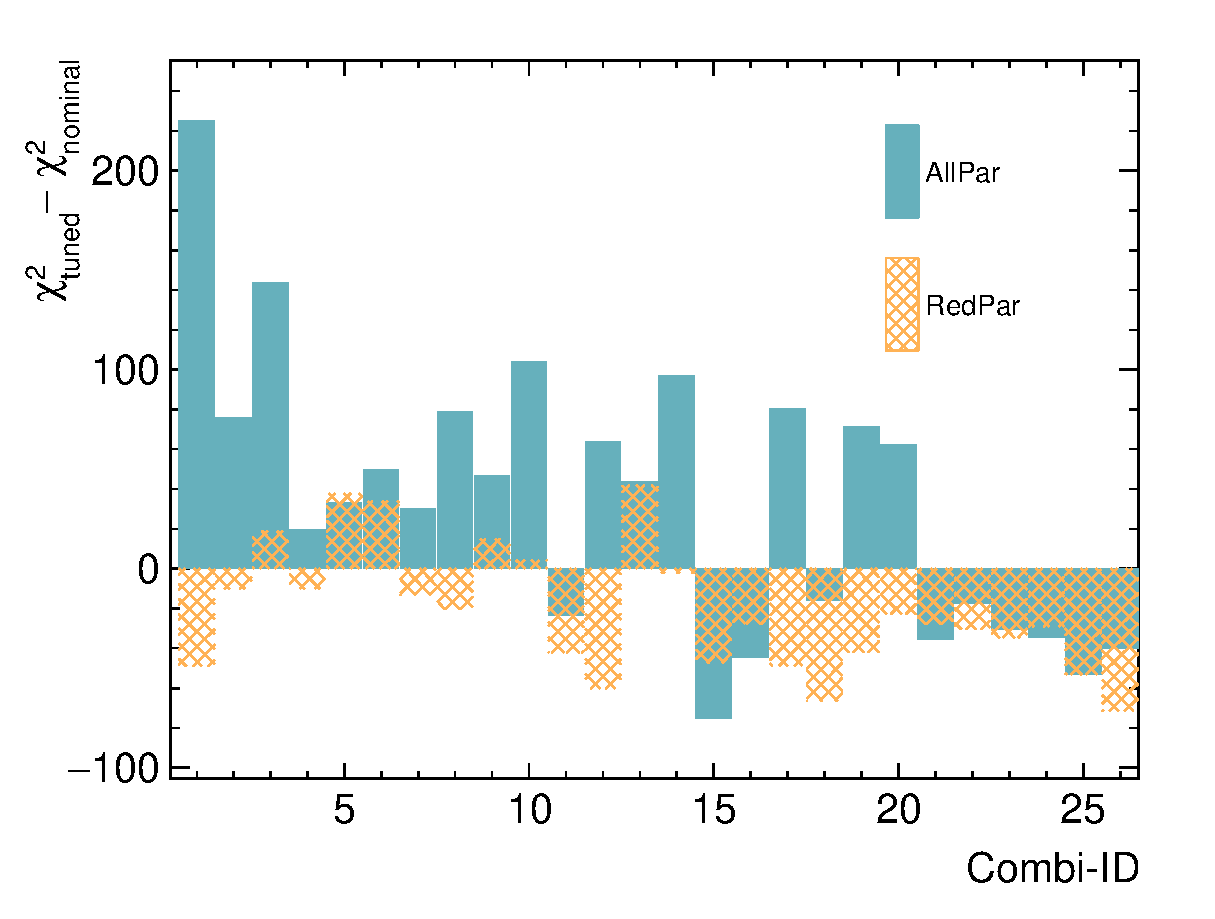
\includegraphics[width=0.45\textwidth]{fig/chi2_hist.eps} 
    \caption{\label{fig:allchi} Change of $\chi^2$ calculated for the full (i.e., tuned plus validation) observable set as a function of the tuned combination. The two model parameter sets (\allpar and \redpar, see Table~\ref{tab:hALFG-para} for definitions) are compared and it can be seen that the respective minima happen at \texttt{Combi-15} and 26. }   
\end{figure}
    
    \subsubsection{\label{sec:tune-results}Tuning Results} 
    Table~\ref{tab:restunes} summarises the tuned parameter values and the $\chi^2$ changes of the best tunes. 
    The tune, \restunefull (\gC), is tuned on the observable set \cbRedPar using \redpar, while the tune, $\alttune$~(\gT), is tuned on \cbAllPar using \allpar. 
    For the \gC tune, changes to the \sfcfg model are moderate ($\srcfr$ increases from $0.12$ to $0.15$), while changes in the hA model are large. More specifically, $\pizmfp$ and $\picex$ are highly suppressed and the nucleon FSI has larger CEX and PIPD and lower ABS.  
    The tune \gT differs most from \gC in $\srcfr$ and $\picex$. 
    The lower part of the table illustrates $\chi^2$ improvements for selected (\texttt{combi}) and non-selected (\texttt{vald}) observables. 
    It is reassuring that both tunes have substantial reduction in the total $\chi^2$ and also in the \texttt{vald}  $\chi^2$.
    
    \begin{table}[!htb]
        \centering
        \begin{tabular}{cccc}
        \hline
        \hline
        Parameter              & Nominal (\gZero) &  \redpar  (\gC)     & \allpar  (\gT)   \\
        \hline
        \multicolumn{4}{c}{\sfcfg} \\
        \hline
        $\srcfr$   & 0.12 & 0.15 $\pm$ 0.08         & 0.30  $\pm$ 0.05       \\
        $\nurmec$  & 0.01 & 0.01                    & 0.011 $\pm$ 0.003     \\
        \hline
        \multicolumn{4}{c}{hA} \\
        \hline
        $\cpimfp$  & $1.0\pm0.2$ & 1.0    & 1.11   $\pm$ 0.16       \\
        $\pizmfp$  & $1.0\pm0.2$ & 0.22 $\pm$ 0.07          & 0.17   $\pm$ 0.06        \\
        $\nmfp$    & $1.0\pm0.2$& 1.0                      & 1.20   $\pm$ 0.12     \\
        \hline
        $\picex$   & $1.0\pm0.5$ & 0.26 $\pm$ 0.12          & 1.53   $\pm$ 0.37        \\
        $\ncex$    & $1.0\pm0.4$ & 1.43 $\pm$ 0.34          & 1.41   $\pm$ 0.38       \\
        \hline
        $\piinel$  & $1.0\pm0.4$ & 1.0                      & 0.67   $\pm$ 0.30        \\
        $\ninel$   & $1.0\pm0.4$ & 1.0                     & 1.26   $\pm$ 0.48       \\
        \hline
        $\cpiabs$  & $1.0\pm0.2$ & 1.0                      & 1.59   $\pm$ 0.31         \\
        $\pizabs$  & $1.0\pm0.2$ & 1.0                      & 0.90   $\pm$ 0.28         \\
        $\nabs$    & $1.0\pm0.2$ & 0.25 $\pm$ 0.28          & 0.28   $\pm$ 0.27       \\
        \hline
        $\pipiprod$& $1.0\pm0.2$ & 1.0                      & 1.12   $\pm$ 0.30     \\
        $\npiprod$ & $1.0\pm0.2$ & 2.05 $\pm$ 0.48          & 1.27   $\pm$ 0.48       \\ 
        \hline
        \hline
        \multicolumn{4}{c}{$\chi^2$ \textrm{for} \texttt{combi}} \\
        \hline
        \texttt{untuned}         & & 231.75         & 161.26        \\
        \texttt{tuned}           & & 174.84         & 122.53        \\
        \texttt{diff}            & & -56.91         & -38.73        \\
        \hline
        \multicolumn{4}{c}{$\chi^2$ \textrm{for} \texttt{vald}} \\
        \hline
        \texttt{untuned}    & & 229.5          & 299.99        \\
        \texttt{tuned}            & & 214.7          & 263.41        \\
        \texttt{diff}       & & -14.8          & -36.58        \\
        \hline
        \multicolumn{4}{c}{$\chi^2$ \textrm{for} \texttt{combi+vald}} \\
        \hline
        \texttt{untuned}    & &  461.25          &  461.25        \\
        \texttt{tuned}          &  & 389.54 & 385.94        \\
        \texttt{diff} & & -71.71         & -75.31  \\     
        \hline
        \hline
    \end{tabular}
    \caption{\label{tab:restunes}
    	Parameters in \gZero, \gC, and \gT. Those without errors are not tuned. Lower section: \texttt{combi} indicates that the following $\chi^2$ sums are calculated for the tuned measurements (i.e. \cbRedPar (98 bins) and \cbAllPar (72 bins) for \gC and \gT, respectively), while \texttt{vald} indicates that the respective validation sets are used; \texttt{untuned} means that the $\chi^2$ calculation uses the nominal values of the parameters, while \texttt{tuned} denotes the tuned ones. \texttt{diff} displays the improvement achieved by the respective tuning.  
    }
    \end{table}
    
    To further investigate the tuning impacts, predictions for $\pn$ using \gZero and \gC are plotted in Fig.~\ref{fig:g24-c-pn-reac}. 
    For \ttkzpi, \ttkpip and \minzpi, the new $\chi^2$ values are comparable to those obtained with \gZero, changing less than the number of bins. 
    For \minpiz, \gC is distinctly better than \gZero, thereby demonstrating the possibility of simultaneous good descriptions of both pion-less and pion production samples with constrained parameters from cross-topology TKI tuning.

    \begin{figure*} 
        \centering 		
        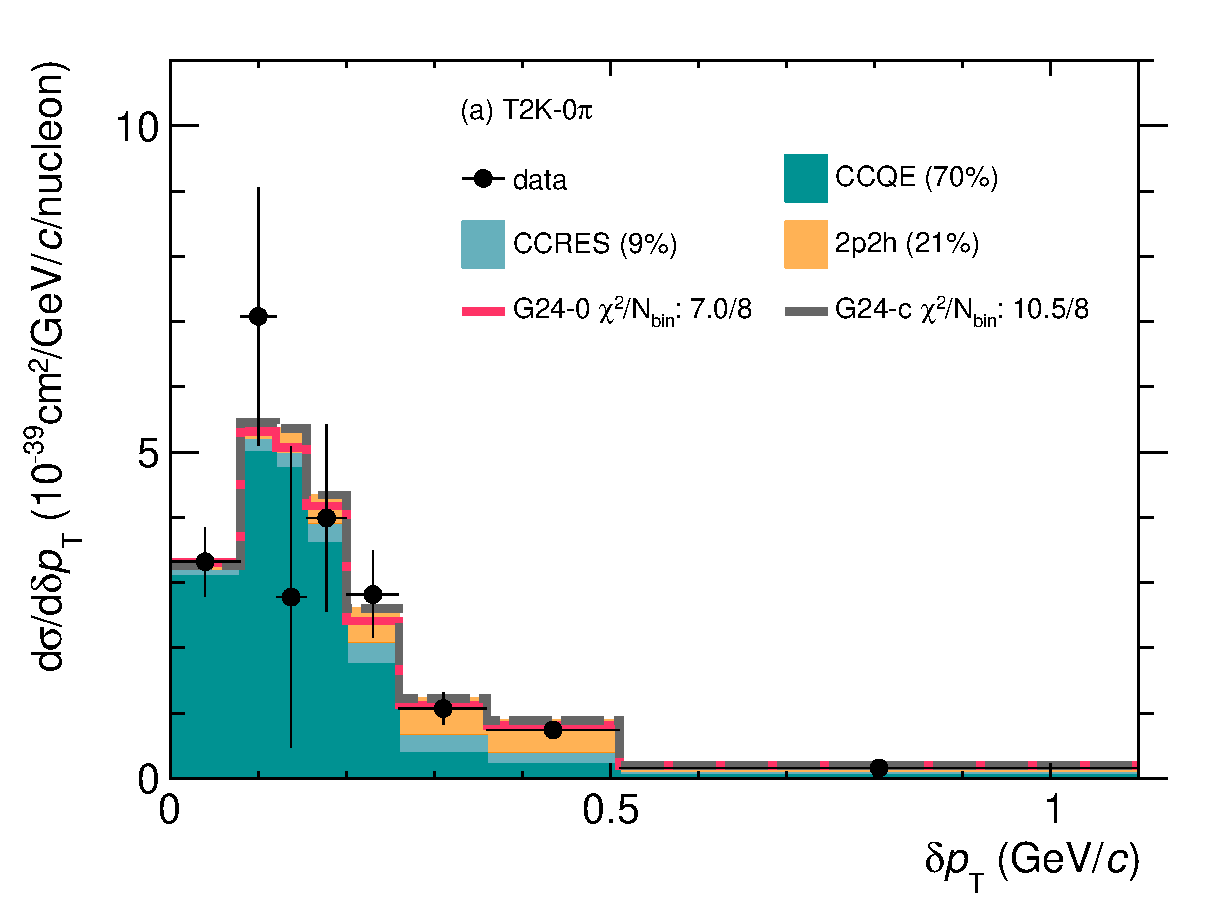
\includegraphics[width=0.23\textwidth]{fig/0026-t2k_0pi_dpt_reac_decomp.eps}
        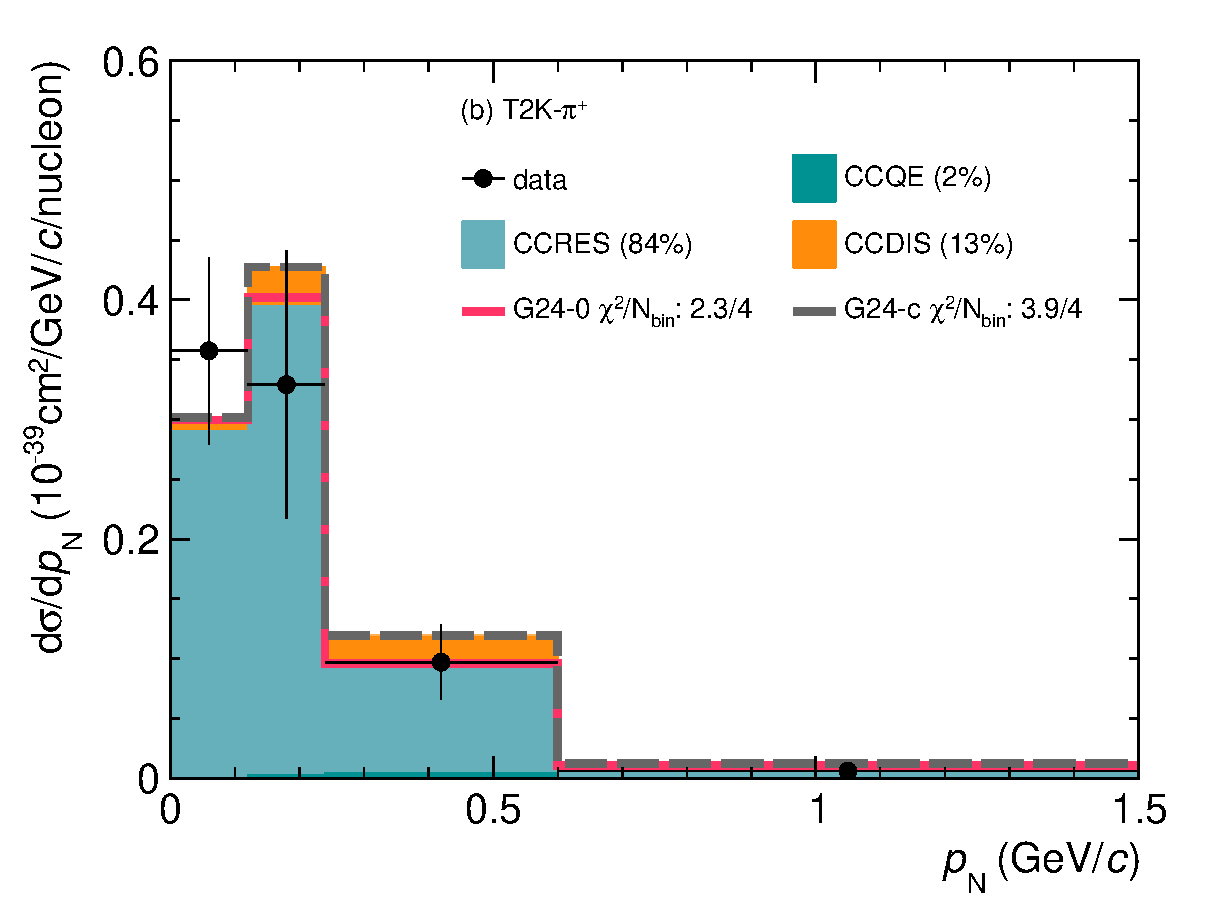
\includegraphics[width=0.23\textwidth]{fig/0026-t2k_pip_pn_reac_decomp.eps}	
        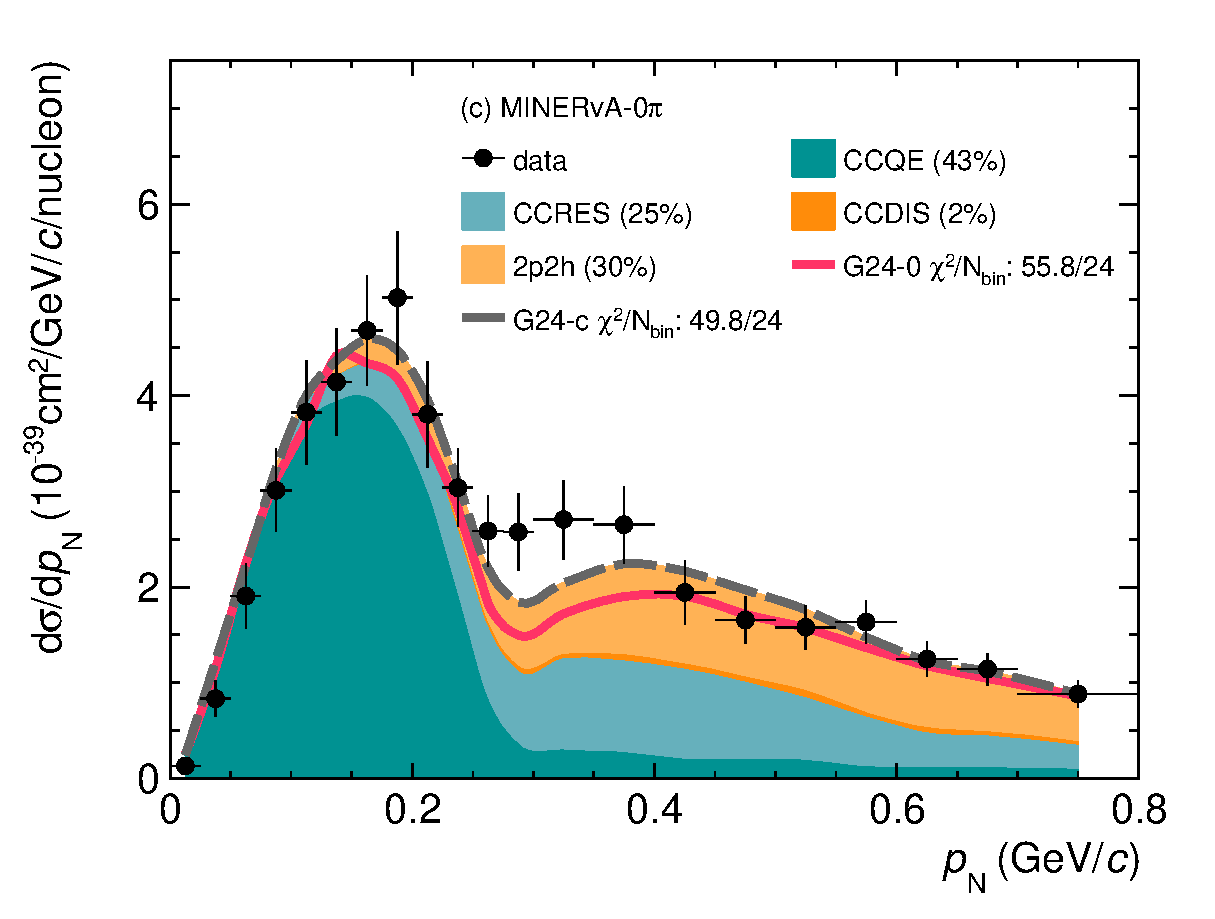
\includegraphics[width=0.23\textwidth]{fig/0026-min_0pi_pn_reac_decomp.eps}
        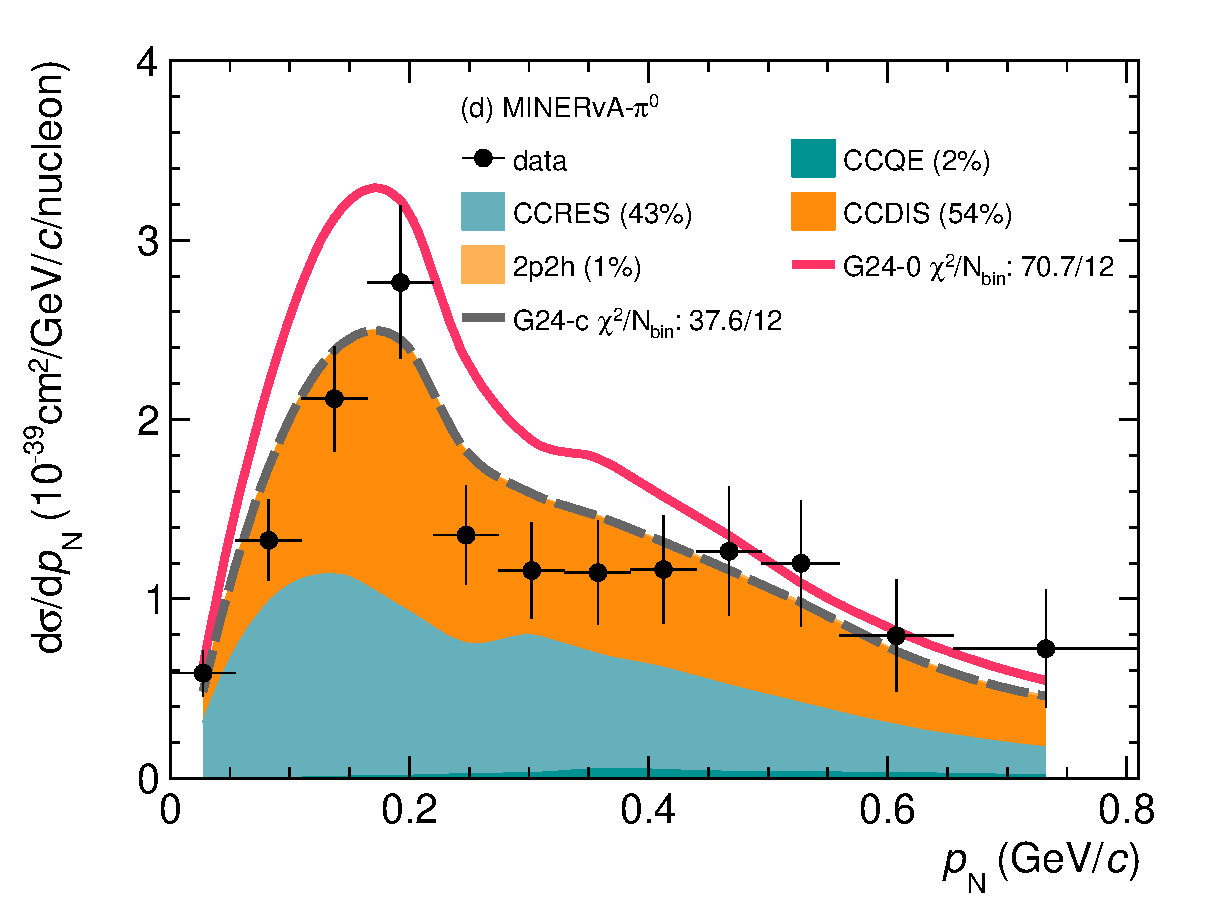
\includegraphics[width=0.23\textwidth]{fig/0026-min_pi0_pn_reac_decomp.eps}
        \caption{\label{fig:g24-c-pn-reac}  
        Comparisons of predictions for $\pn$ using \gZero and \gC. 
        } 
    \end{figure*}

    To understand better the origin of the improvement, the decomposition of the cross section for $\dat$ according to the FSI fates of the $\piz$ is presented in Fig.~\ref{fig:CEX-minpiz-dat-pi0}.
    Comparing Fig.~\ref{fig:CEX-minpiz-dat-pi0}b to Fig.~\ref{fig:CEX-minpiz-dat-pi0}a, it is evident that the decrease in the cross-section for \gC can be mainly attributed to the considerable reduction in ``No Interaction'' and CEX.
    This matches the tuned parameter values as shown in Table~\ref{tab:restunes}.
    The number of $\piz$s undergoing no FSI (``No Interaction'') is reduced by the suppression of the $\pizmfp$ parameter, while the CEX reduction is caused by the decreased $\picex$.
    \begin{figure}[!htb] 	
        \centering 		
        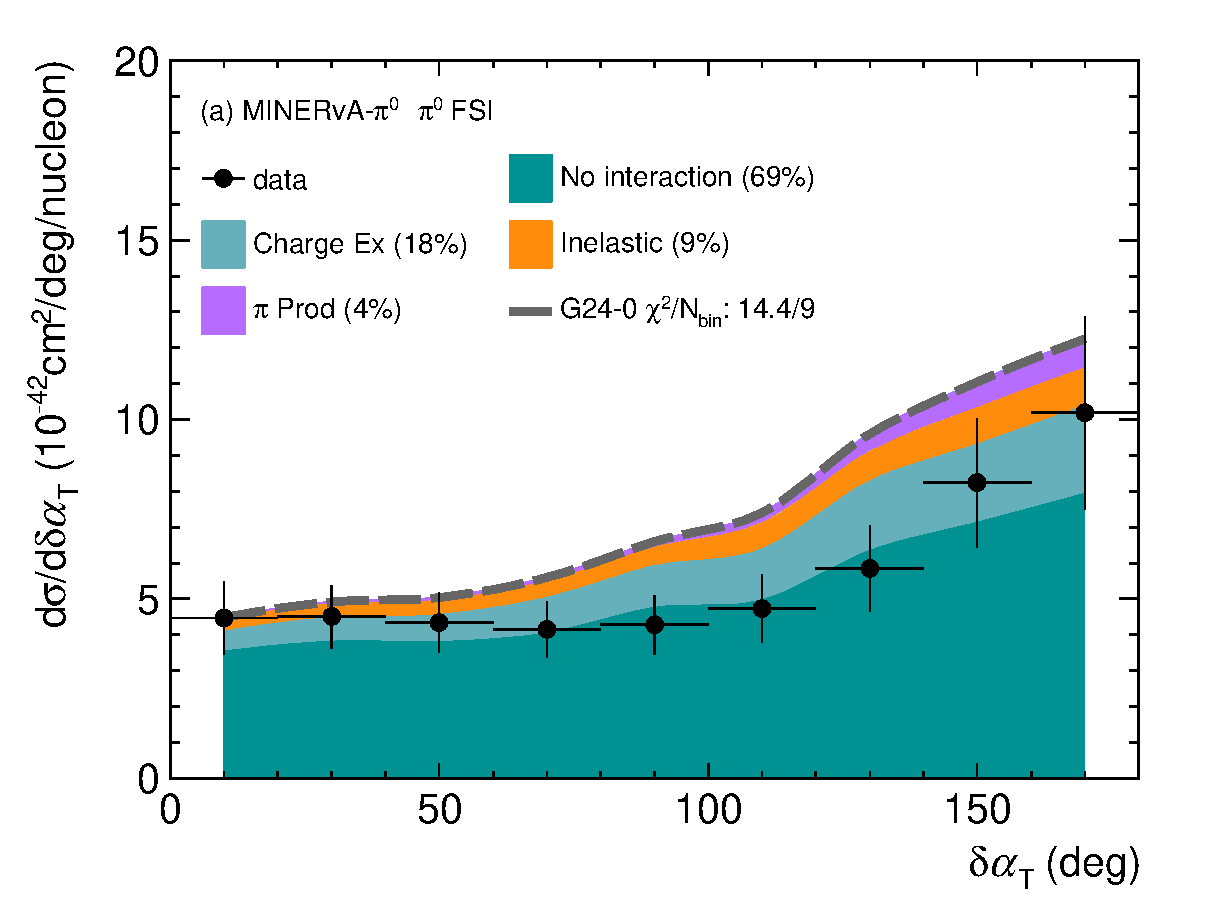
\includegraphics[width=0.45\textwidth]{fig/0000-min_pi0_dalphat_pi0_decomp_cex.eps}
        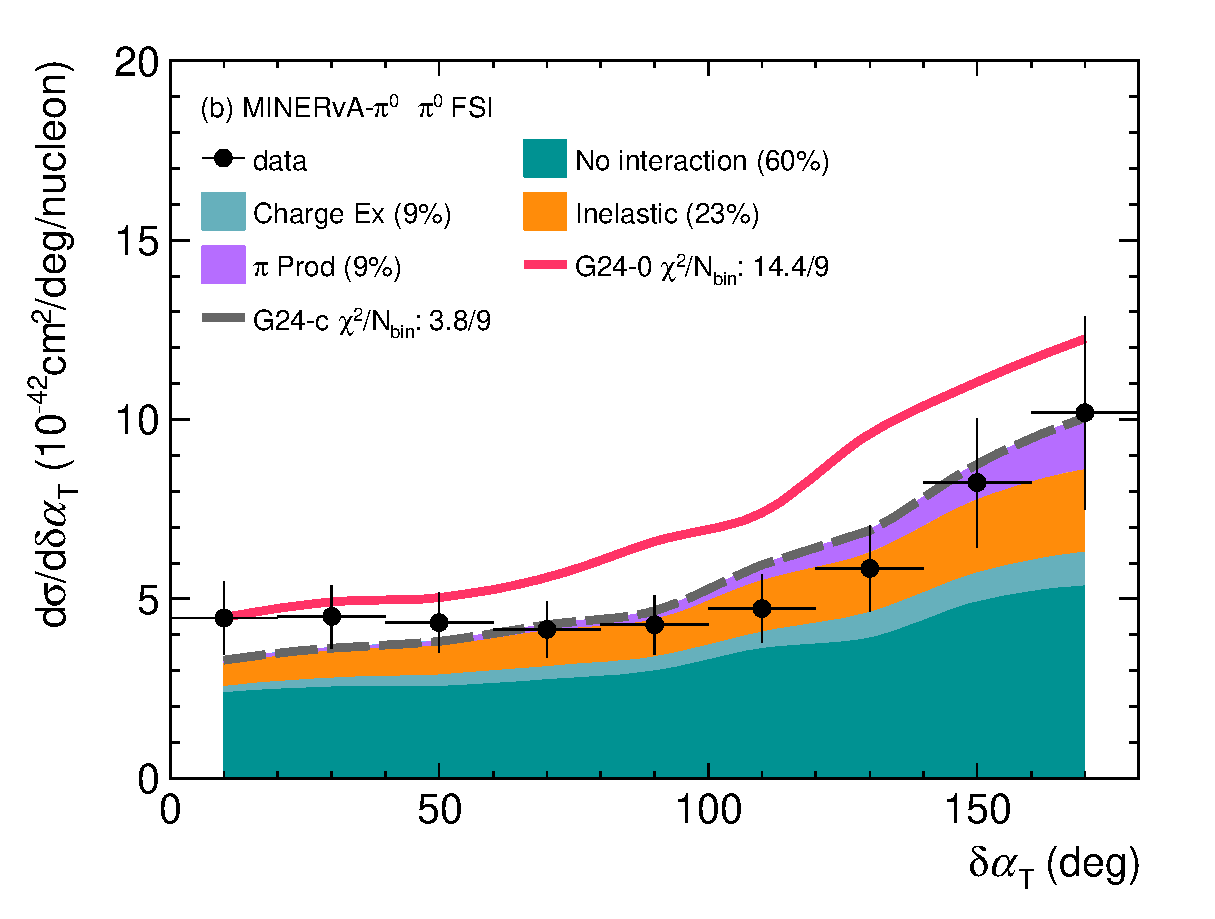
\includegraphics[width=0.45\textwidth]{fig/0026-min_pi0_dalphat_pi0_decomp_cex.eps}	
        \caption{\label{fig:CEX-minpiz-dat-pi0} \minpiz $\dat$ measurement compared to \genie predictions decomposed in $\piz$ FSI fates with (a) \gZero and (b) \gC.} 
    \end{figure}
    In contrast, the impact of these two parameters on the other data sets are relatively small.
    An increase in $\piz$ rescattering can only manifest in pion-less data sets through ABS. 
    There is indeed an increase of ABS for $\piz$ in \ttkzpi and \minzpi, but as the initial fraction is small, the overall impact is insignificant. 
    The increase of $\piz$ rescattering can increase \ttkpip via CEX. 
    However, due to the significant suppression of CEX as discussed below, its impact on \ttkpip is also minimal. 
    
    As for the change of $\picex$, it does not impact \ttkzpi and \minzpi as CEX only changes the pion type without removing them.
    Hence, events with pions in the final state would be rejected in these two data sets regardless of the pion charge. 
    In principle, CEX will also move events from signal to background for \ttkpip when a $\piz$ is converted to a $\pip$ and vice verse. 
    However, \ttkpip does not have a considerable CEX contribution to start with, so changing CEX will also have minimal impacts. 
    Lastly, although $\piinel$ and $\pipiprod$ are not modified explicitly, both INEL and PIPD in \minpiz increase  considerably due to the intricate correlation between the FSI fates in the hA implementation,. 
    Overall, suppressing both ``No Interaction'' and CEX for $\piz$ adjusts the \minpiz prediction to the appropriate magnitude with small impacts on other data sets.  
    
    The effects of the other parameter changes are more transparent in the comparison of the $\pn$ distribution of \minpiz between Figs.~\ref{fig:minpiz-pn-pr}a and~\ref{fig:minpiz-pn-pr}b.
    A relatively large increase in $\ncex$ and $\npiprod$ moves events away from the Fermi motion peak at $\pn\leq0.25~\textrm{GeV}/c$. 
    \begin{figure}[!htb] 	
        \centering 		
        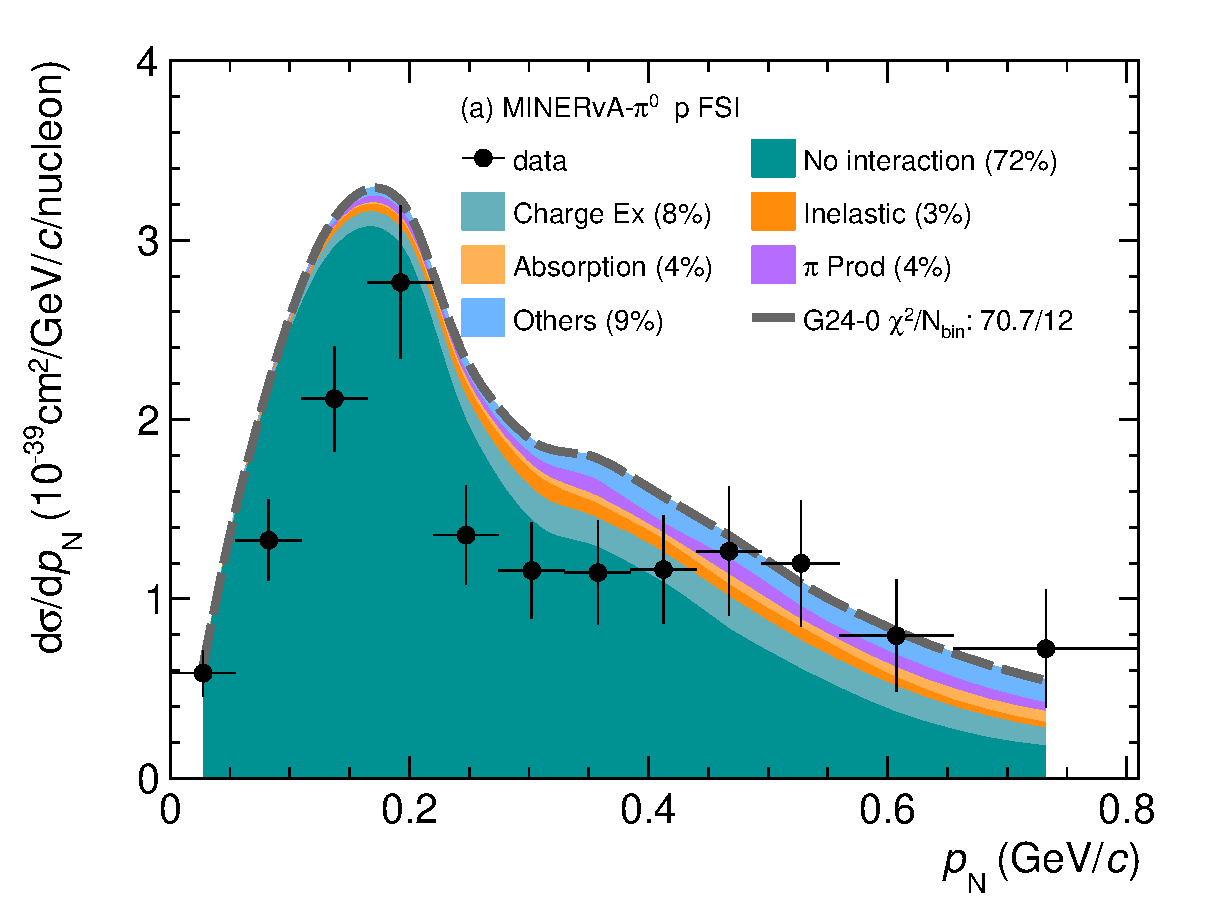
\includegraphics[width=0.45\textwidth]{fig/0000-min_pi0_pn_pr_decomp_cex.eps}
        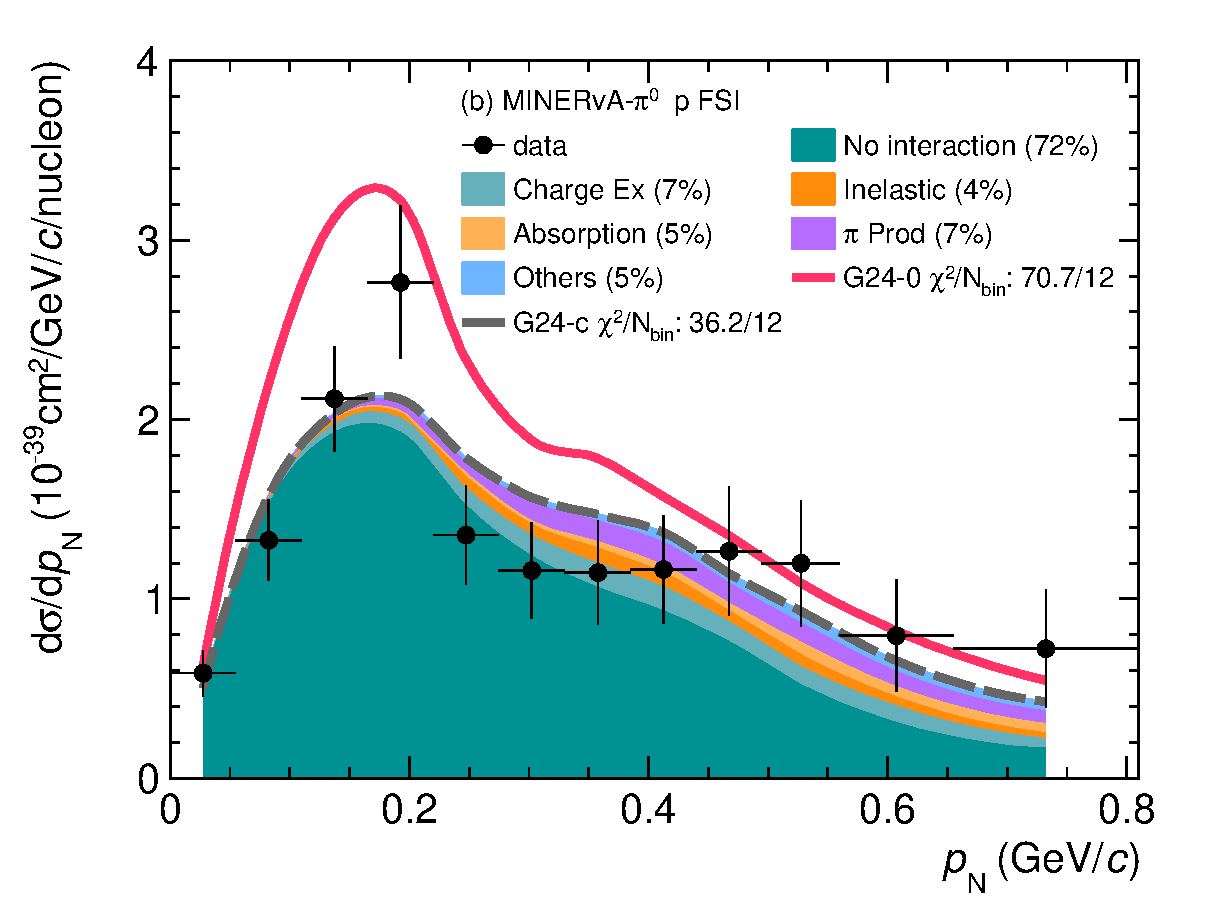
\includegraphics[width=0.45\textwidth]{fig/0026-min_pi0_pn_pr_decomp_cex.eps}	
        \caption{\label{fig:minpiz-pn-pr} Similar to Fig.~\ref{fig:CEX-minpiz-dat-pi0} but for $\pn$ with proton FSI fate decomposition. Note that the ``Absorption'' of the proton is referring to the absorption of the $\pip$ from the decay of $\deltapp$, which could lead to emission of nucleons.     
        } 
    \end{figure}
    This same effect is achieved in the intermediate tune, \gT, by a notable enhancement of $\srcfr$, as illustrated in Fig.~\ref{fig:minpiz-alttune}, which raises the high momentum tail of the nucleon Fermi motion and thus increases RES/DIS (Fig.~\ref{fig:minpiz-alttune}a) ratio.
    Instead of suppressing $\picex$ like \gC, this tune significantly increases it (Fig.~\ref{fig:minpiz-alttune}b) to offset the large reduction of ``No Interaction'' $\piz$ events due to the more suppressed $\pizmfp$ (cf. Table~\ref{tab:restunes}).  
    Overall, this leads to a reduction of $75.31$ in $\chi^2$ (Table~\ref{tab:restunes}), similar to \gC, as well as a good data-MC agreement across all data sets. 
    
    \begin{figure}[!htb] 	
        \centering 		
        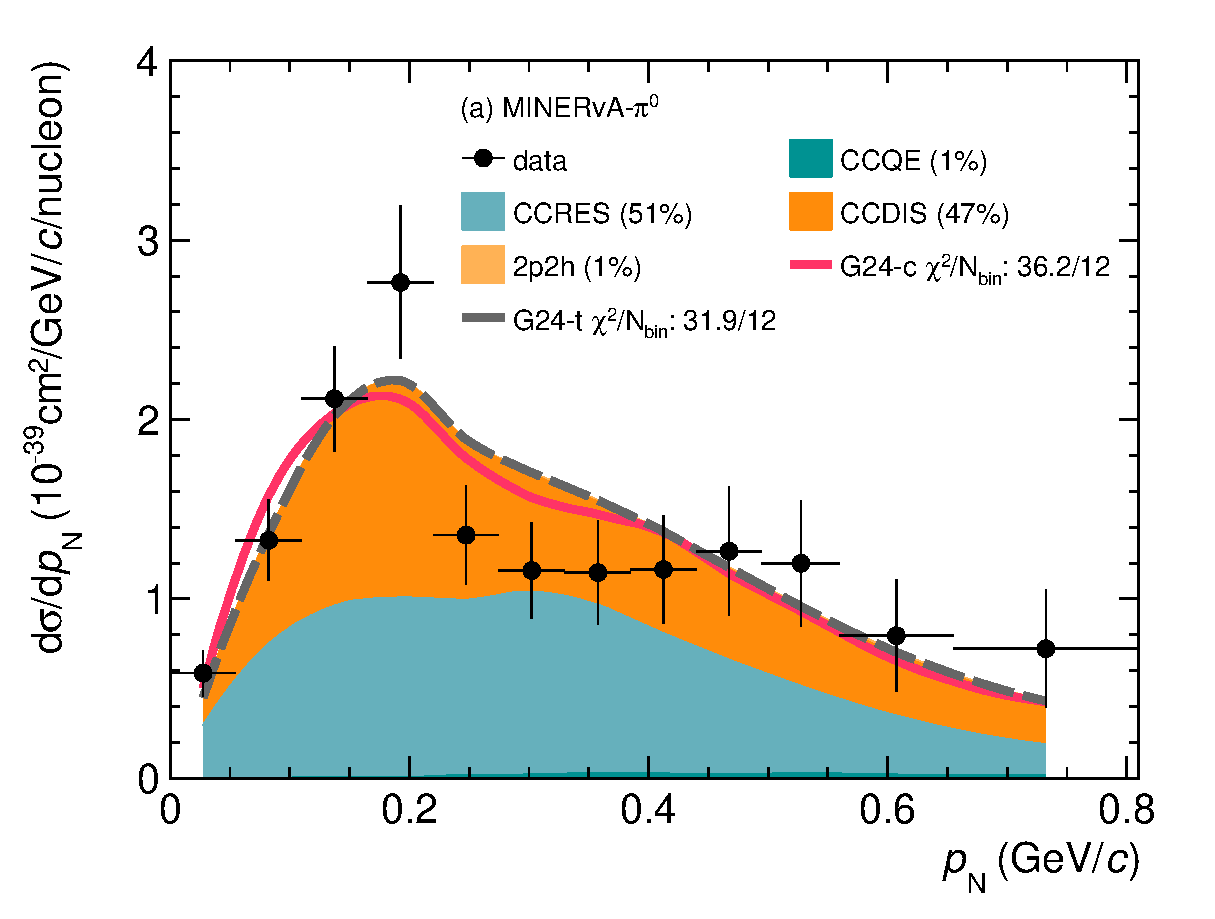
\includegraphics[width=\fwid\textwidth]{fig/0015-min_pi0_pn_reac_decomp_comp.eps}
        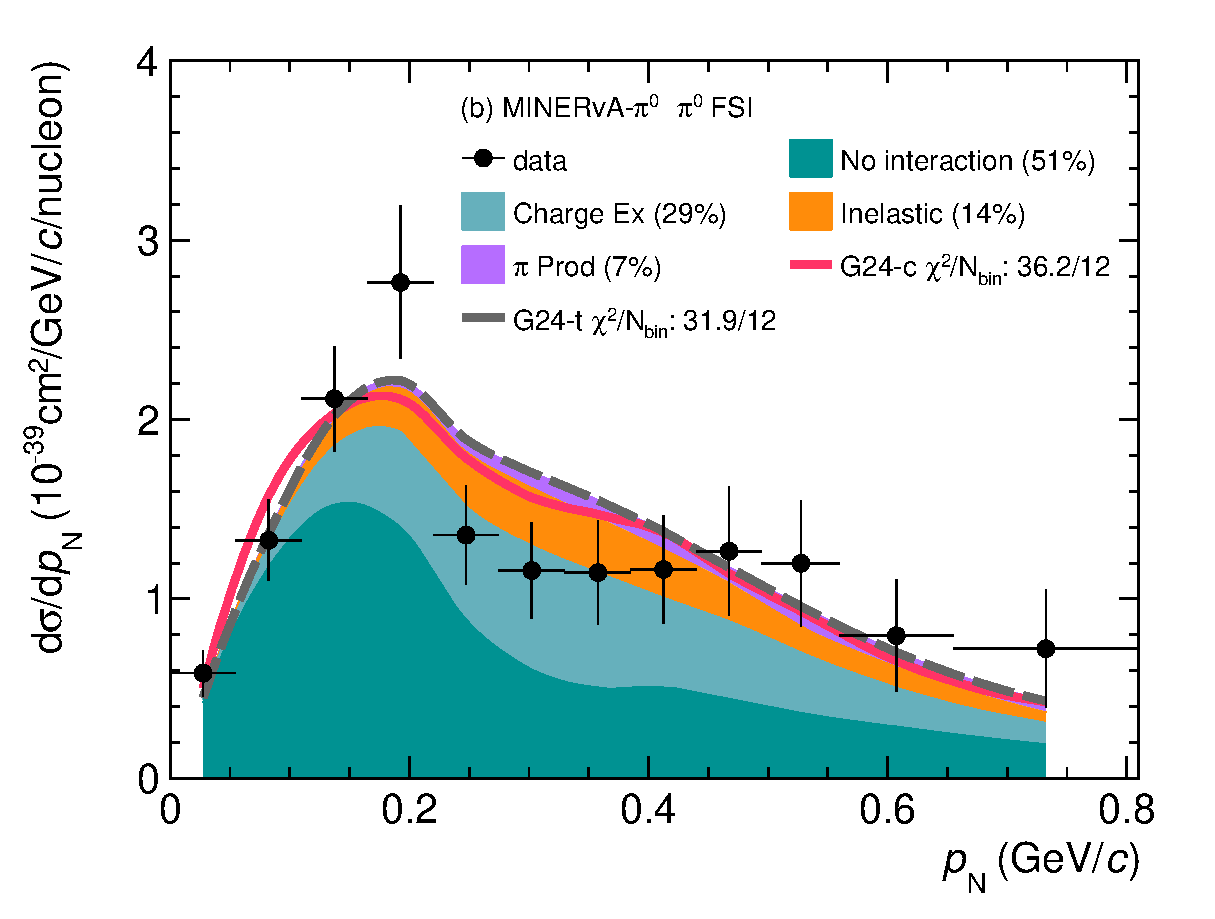
\includegraphics[width=\fwid\textwidth]{fig/0015-min_pi0_pn_pi0_decomp_comp.eps}
        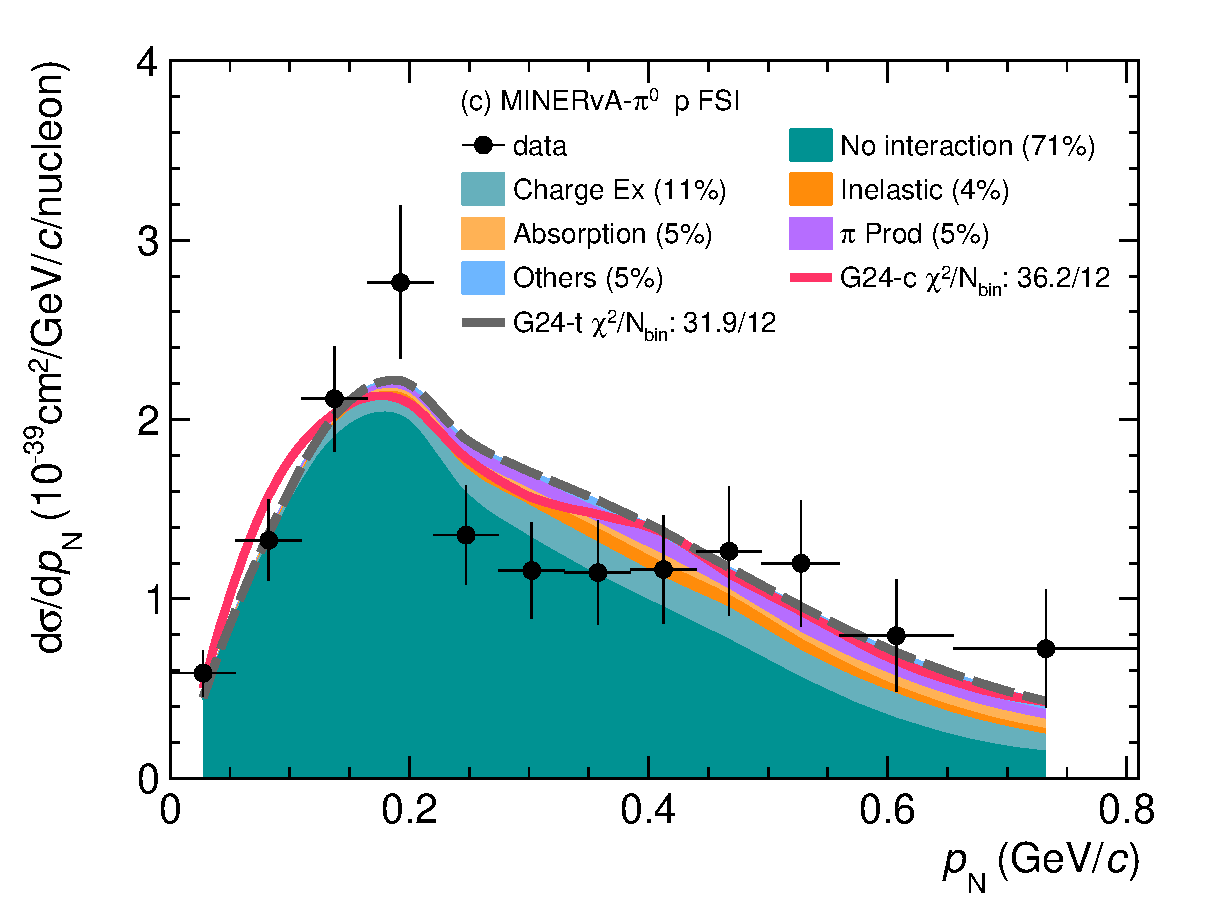
\includegraphics[width=\fwid\textwidth]{fig/0015-min_pi0_pn_pr_decomp_comp.eps}
        \caption{\label{fig:minpiz-alttune} \minpiz $\pn$ measurement compared to \genie predictions decomposed in  (a) $\nu$-N interaction, (b) $\piz$ FSI, and (c) proton FSI for the alternative tune, \gT.} 
    \end{figure}
    
    \subsection{Discussion}
    For both \gC and \gT the fit results suggest extreme values, but the effect of the parameter change is less effective than the change in the parameter suggests. 
    Due to the re-normalisation step after scaling, the effective change for one particular fate is smaller than the corresponding scaling factor. 
    As for the total FSI cross sections adjusted by the MFP scaling parameter, only that of $\piz$ is changed. 
    The total $\piz$-C scattering cross section for pion kinetic energy is plotted in Fig.~\ref{fig:pizmfp_change} to assess the effective impact. 
    The shape remains similar and consistent with Fig. 2.23 ($\pip$-C reactions) in Ref.~\cite{Andreopoulos:2015wxa} while the peak magnitude increases by $48\%$, from $380$ to $538$ mb, which is much less than the scaling factor, $\pizmfp=0.22$, seemingly suggests. 
    Moreover, the default values of $\piz$ parameters are calculated from charged pion data assuming isospin symmetry due to the lack of $\piz$ experimental data. 
    Hence, this modification does not violate any  agreement with existing hadron scattering data.
    \begin{figure}[!htb] 	
        \centering 		
        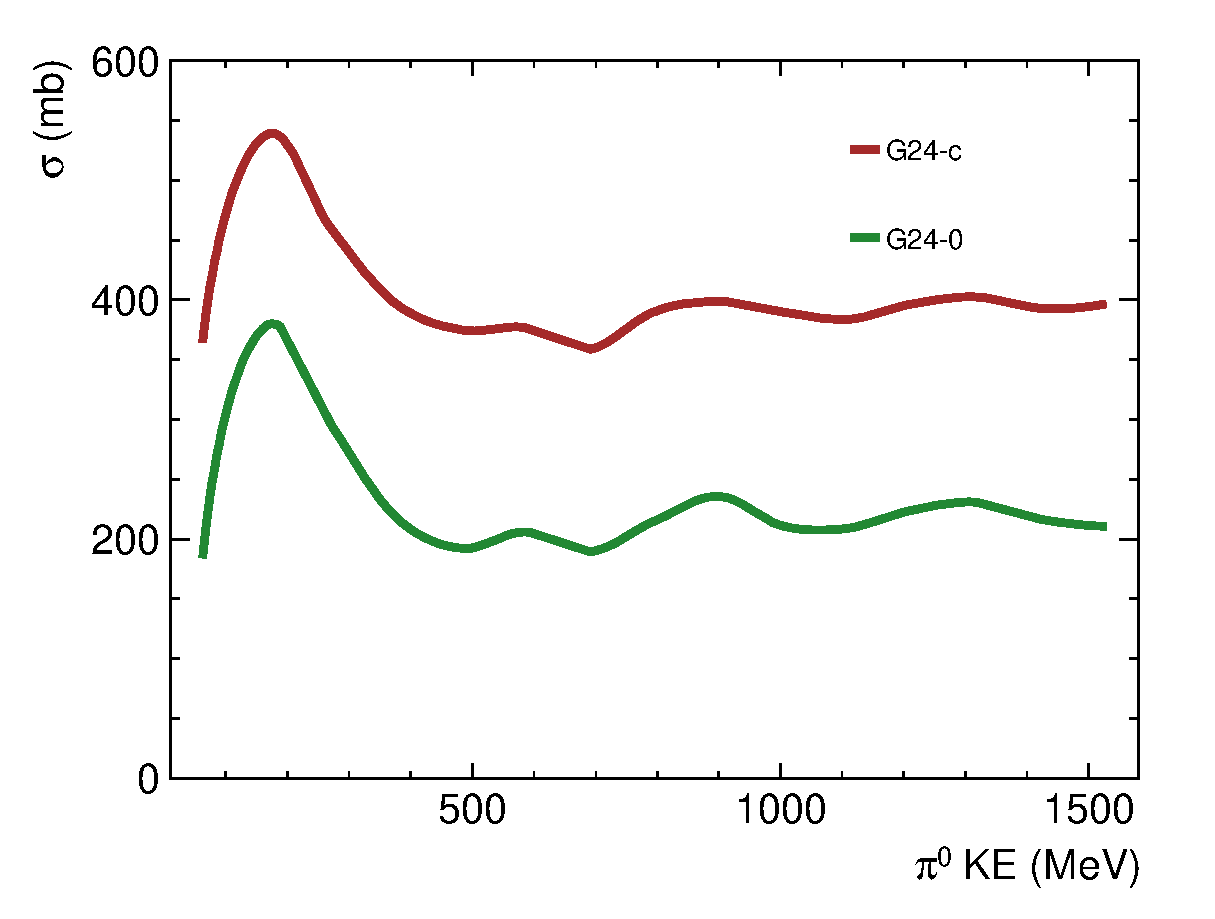
\includegraphics[width=\fwid\textwidth]{fig/pi0mfp_change.eps}
        \caption{\label{fig:pizmfp_change} Change in MC prediction for $\piz$ cross section between \gZero and \gC . } 
    \end{figure}
    
    Besides, agreement of this tune with most of the non-TKI neutrino datasets available is unchanged before and after the tune,  thereby bolstering the physicality of the tune. 
    In conclusion, this tune is an effective model, suitable as a starting point for an analysis. 
    Further refinement will be possible once more data, including non-TKI observables, are included in the fit. 

